%% Manuscript for the effect of designed conversational architecture on the perception of agents
%%
%% The first command in your LaTeX source must be the \documentclass command.
\documentclass[sigconf,screen]{config/acmart}

%\usepackage[linewidth=1pt]{mdframed}
\usepackage{lipsum}
\usepackage{multirow}
\usepackage{graphicx}
\usepackage{booktabs}
\usepackage{makecell} 
\usepackage{stfloats}
\usepackage{longtable}

\newcommand{\cmt}[1]{}%{\ignorespaces}

\usepackage{soul}
\usepackage{color}
\newcommand{\hlrev}[1]{{\sethlcolor{yellow}\hl{#1}}}

%% NOTE that a single column version may be required for 
%% submission and peer review. This can be done by changing
%% the \doucmentclass[...]{acmart} in this template to 
%% \documentclass[manuscript,screen]{acmart}
%% 
%% To ensure 100% compatibility, please check the white list of
%% approved LaTeX packages to be used with the Master Article Template at
%% https://www.acm.org/publications/taps/whitelist-of-latex-packages 
%% before creating your document. The white list page provides 
%% information on how to submit additional LaTeX packages for 
%% review and adoption.
%% Fonts used in the template cannot be substituted; margin 
%% adjustments are not allowed.
%%
%%
%% \BibTeX command to typeset BibTeX logo in the docs
\AtBeginDocument{%
  \providecommand\BibTeX{{%
    \normalfont B\kern-0.5em{\scshape i\kern-0.25em b}\kern-0.8em\TeX}}}

\copyrightyear{2023} 
\acmYear{2023} 
\setcopyright{acmlicensed}\acmConference[CUI '23]{ACM conference on Conversational User Interfaces}{July 19--21, 2023}{Eindhoven, Netherlands}
\acmBooktitle{ACM conference on Conversational User Interfaces (CUI '23), July 19--21, 2023, Eindhoven, Netherlands}
\acmPrice{15.00}
\acmDOI{10.1145/3571884.3597139}
\acmISBN{979-8-4007-0014-9/23/07}

%% Rights management information.  This information is sent to you
%% when you complete the rights form.  These commands have SAMPLE
%% values in them; it is your responsibility as an author to replace
%% the commands and values with those provided to you when you
%% complete the rights form.
%\setcopyright{acmcopyright}
%\copyrightyear{2023}
%\acmYear{2023}
%\acmDOI{3571884.3597139}

%% These commands are for a PROCEEDINGS abstract or paper.
%\acmConference[Conference acronym 'XX]{Make sure to enter the correct
%  conference title from your rights confirmation email}{June 03--05,
%  2018}{Woodstock, NY}
%
%  Uncomment \acmBooktitle if th title of the proceedings is different
%  from ``Proceedings of ...''!
%
%\acmBooktitle{Woodstock '18: ACM Symposium on Neural Gaze Detection,
%  June 03--05, 2018, Woodstock, NY} 
%\acmPrice{15.00}
%\acmISBN{978-1-4503-XXXX-X/18/06}

%%
%% Submission ID.
%% Use this when submitting an article to a sponsored event. You'll
%% receive a unique submission ID from the organizers
%% of the event, and this ID should be used as the parameter to this command.
%%\acmSubmissionID{123-A56-BU3}

%%
%% end of the preamble, start of the body of the document source.
\begin{document}
%TC:ignore

%%
%% The "title" command has an optional parameter,
%% allowing the author to define a "short title" to be used in page headers.
% \title[short title]{How to Make Pinocchio a Real Boy? Designing conversational architecture elements to achieve desirable anthropomorphized perceptions}
\title{The Bot on Speaking Terms: The Effects of Conversation Architecture on Perceptions of Conversational Agents}

%%
%% The "author" command and its associated commands are used to define
%% the authors and their affiliations.
%% Of note is the shared affiliation of the first two authors, and the
%% "authornote" and "authornotemark" commands
%% used to denote shared contribution to the research.
\author{Christina Wei}
\email{christina.wei@mail.utoronto.ca}
\affiliation{%
  \institution{University of Toronto}
  \city{Toronto}
  \country{Canada}
}

\author{Young-Ho Kim}
\email{yghokim@younghokim.net}
\affiliation{%
  \institution{NAVER AI Lab}
  \country{Republic of Korea}
}

\author{Anastasia Kuzminykh}
\email{anastasia.kuzminykh@utoronto.ca}
\affiliation{%
  \institution{University of Toronto}
  \city{Toronto}
  \country{Canada}
}

%%
%% By default, the full list of authors will be used in the page
%% headers. Often, this list is too long, and will overlap
%% other information printed in the page headers. This command allows
%% the author to define a more concise list
%% of authors' names for this purpose.
\renewcommand{\shortauthors}{Wei, Kim, Kuzminykh} %It will be automatically anonymized through the document class property anonymous

%%
%% The abstract is a short summary of the work to be presented in the
%% article.

\begin{abstract}
Conversational agents mimic natural conversation to interact with users. Since the effectiveness of interactions strongly depends on users’ perception of agents, it is crucial to design agents’ behaviors to provide the intended user perceptions. Research on human-agent and human-human communication suggests that speech specifics are associated with perceptions of communicating parties, but there is a lack of systematic understanding of how speech specifics of agents affect users' perceptions. To address this gap, we present a framework outlining the relationships between elements of agents’ conversation architecture (dialog strategy, content affectiveness, content style and speech format) and aspects of users’ perception (interaction, ability, sociability and humanness). Synthesized based on literature reviewed from the domains of HCI, NLP and linguistics (n=57), this framework demonstrates both the identified relationships and the areas lacking empirical evidence. We discuss the implications of the framework for conversation design and highlight the inconsistencies with terminology and measurements.
\end{abstract}

%%
%% The code below is generated by the tool at http://dl.acm.org/ccs.cfm.
%% Please copy and paste the code instead of the example below.
%%
\begin{CCSXML}
<ccs2012>
   <concept>
       <concept_id>10003120.10003121.10003126</concept_id>
       <concept_desc>Human-centered computing~HCI theory, concepts and models</concept_desc>
       <concept_significance>500</concept_significance>
       </concept>
   <concept>
       <concept_id>10003120.10003121.10003122</concept_id>
       <concept_desc>Human-centered computing~HCI design and evaluation methods</concept_desc>
       <concept_significance>500</concept_significance>
       </concept>
   <concept>
       <concept_id>10003120.10003121.10003124.10010870</concept_id>
       <concept_desc>Human-centered computing~Natural language interfaces</concept_desc>
       <concept_significance>500</concept_significance>
       </concept>
 </ccs2012>
\end{CCSXML}

\ccsdesc[500]{Human-centered computing~HCI theory, concepts and models}
\ccsdesc[500]{Human-centered computing~HCI design and evaluation methods}
\ccsdesc[500]{Human-centered computing~Natural language interfaces}

%%
%% Keywords. The author(s) should pick words that accurately describe
%% the work being presented. Separate the keywords with commas.
\keywords{conversational agents, natural language interface, chatbots, virtual assistants, user perceptions, anthropomorphized perceptions, conversation architecture, speech variations}

%%\received{20 February 2007}
%%\received[revised]{12 March 2009}
%%\received[accepted]{5 June 2009}

%%
%% This command processes the author and affiliation and title
%% information and builds the first part of the formatted document.
\maketitle
%TC:endignore

%% INTRODUCTION SECTION %%

\section{Introduction}

Conversational agents (CAs), such as Amazon Alexa or Google Assistant, are designed to interact with humans using natural language through voice or text modalities. Since these agents communicate in natural language, the effectiveness of interactions between users and conversational agents in achieving users' goals depend heavily on the \textit{conversation architecture}, which refers to the content and manner of communication utilized by the agents \mbox{\cite{knijnenburg2016inferring, seeger2021chatbots}}.
%\textit{conversation architecture}---what and how a CA says---affects users' perceptions of agents and, in turn, the effectiveness of their interactions with users \cite{knijnenburg2016inferring, seeger2021chatbots}, i.e. supporting users in achieving their goals. 
%For instance, p
Previous research suggests that there is a relationship between CAs' conversation architecture and how users perceive these agents %.
%While various studies investigated how some elements of conversation architecture affect users' perceptions of agents~
(e.g.,~\cite{clark2019state, feine2019taxonomy, finch2020towards}).  
%\hlrev{However, there is currently a lack of overall comprehension of the relationship between users' perceptions and conversation architecture elements, specifically which elements are significant and how they impact these perceptions.}
%However, there is currently a lack of systematic understanding of these relationships, i.e. what elements of conversation architecture are impactful for users' perceptions and how they impact these perceptions. 
While various studies investigated how some elements of conversation architecture affect aspects of users' perceptions or discussed the speech specifics of agents as part of a broader analysis of the state of research \cite{clark2019state,feine2019taxonomy}, there is no comprehensive analysis of %research specifically for 
conversation architecture elements that are relevant to user perceptions. 
As such, this paper aims to provide a systematic understanding of the effect of conversation architecture elements on users' perceptions of conversational agents. Such an understanding is essential for guiding the design of conversation architecture, which would allow us to both predict and develop users' appropriate perceptions of agents.

%there is a lack of systematic understanding of these relationships.
%paucity of knowledge on the overall coverage and effects of these relationships explored in literature. 
%One reason for this disparity is, arguably, the lack of clear and consistent definitions of both the aspects of users' perceptions of agent and conversation architectural elements. Although some authors discuss the speech specifics of agents as part of a broader analysis on the state of research \cite{clark2019state,feine2019taxonomy}, there is no comprehensive analysis of %research specifically for 
%conversation architecture elements that are relevant to user perceptions. Similarly for user perceptions, while there is some research exploring the perceptions of agents as part of understanding the user experiences \cite{clark2019state, finch2020towards} or social cues \cite{feine2019taxonomy} of CAs, there is no exhaustive research specifically for perceptions of agents that are affected by conversation architecture elements. 

%These research gaps related to the paucity of knowledge on synthesizing the effect of speech specifics on perceptions of CAs as well as the lack of systematic understanding on the elements of conversation architecture and perceptions of agents 

%To address this gap, %in this paper, we
%we aim to understand how to design conversation architecture in order to orchestrate perceptions of conversational agents.
%First, we 
To gain this systematic understanding, we explored the following research questions in this paper: \textbf{(RQ1) what aspects of users' perceptions of agents have been explored in relation to the effects of conversation architecture elements?}, \textbf{(RQ2) what elements of conversation architecture are relevant to users' perceptions of agents?}, and \textbf{(RQ3) what is known about the specifics of these relationships between conversation architecture elements and the perceptions of CAs?}
%While there are various elements of conversation architecture used in a CA's utterances, we don't have a systematic understanding of them. This leads to our second research question: \textbf{(RQ2) what elements of conversation architecture are relevant to users' perceptions of agents?} Lastly, we want to understand the effect of conversation architecture on perceptions of agent, specifically: \textbf{(RQ3) what are the relationships between conversation architecture elements and the perceptions of CAs?}
In order to answer these questions, we performed a comprehensive review of the existing literature published from 2010 to 2022 and synthesized the effect of conversation architecture elements on the perceptions of CAs based on the final dataset of 57 relevant papers (\autoref{fig:heatmap_identified}). Based on this review, we grouped the perceptions of agents that were shown to be affected by conversation architecture into four categories (interaction, ability, sociability and humanness) and eleven aspects (\autoref{tbl:perceptions}), and grouped the speech variations related to perceptions of agents into four categories (dialog strategy, content affectiveness, content style and speech format) and eleven elements (\autoref{tbl:conversation_architecture}). 
We found that perceptions of interaction with CAs (usability, engagement, satisfaction) have been most explored in relation to speech variations, while the perceptions of CAs' ability (intelligence, competence, credibility) have been explored the least.
%the least number of explored and identified relationships. 
Our results also show that the conversation architecture elements of response delay and agent-initiated dialog related to perceptions of CAs are under-explored in literature. 
Thus, our work contributes to the CUI community by presenting a framework that synthesizes the findings on the effect of conversation architecture on perceptions of conversational agents while also identifying and clustering perception aspects and conversation architecture elements. %, providing clear and consistent terms that can be used in future research. Together, these contributions move us one step closer to designing CAs that effectively interact with users. 

In the remainder of the paper, we first outline related background work, then describe the literature review process and the framework synthesis method, %, the characteristics of the papers in our reviewed corpus. Following that, we 
followed by a detailed description of the taxonomies of the aspects of the perception of agents and conversation architecture elements, as well as the synthesized framework for their relationships. We conclude by discussing the implications of this work, including 
the associated research challenges and opportunities, as well as ethical considerations for designing the conversational architecture to affect users' perceptions of conversational agents.
%% RELATED WORK SECTION %%

\section{Related Work}
%Communication with conversational agents 
Similar to human-human communication, users utilize natural languages when interacting with conversational agents. %human communication with conversational agents relies on natural languages for interaction. 
However, while it is tempting to leverage components from human-human conversation in designing interactions with conversational agents, studies have demonstrated that there are differences between human-human communications and human-agent communications \cite{clark2019makes, hill2015real}. Currently, CAs are considered as a user-controlled tool rather than a social companion, with a focus on the utilitarian aspects of the conversation \cite{clark2019makes}\cmt{[1]}. When conversing with agents, users tend to use shorter messages with limited vocabulary, adapting to the style of the agent \cite{hill2015real}. Also, some studies found that small talk and humour are considered unnecessary or even inauthentic in conversations with CAs, while these elements are important in scaffolding communications with human partners \cite{clark2019makes, doyle2019mapping}\cmt{[1],[2]}. There are also machine-like traits that users preferred in a CA, such as the ability to interact through multimodal media, and a machine's perceived ability to be objective and non-judgemental \cite{doyle2019mapping, kim2022understanding}\cmt{[2],[3]}. Given human-agent communications are different from human-human communications, it is important to look specifically at the design of user experiences for conversational agents.

There are a number of studies investigating factors affecting user experiences for conversational agents, which includes exploring the relationship between conversation architecture elements and agents' perceptions. For instance, the use of affective language is commonly explored, with studies finding that conversational agents are perceived as more socially present and emotionally intelligent if they use sentiment-adaptive responses based on user's utterances \cite{diederich2019emulating, yang2017perceived}. Another commonly explored element is the use of prosody in voice-based agents, such as the use of express prosody contributing to higher perceived enjoyment and intimacy with the agent \cite{kim2020can}. However, there is a paucity of research to synthesize these findings on user experiences with agents across literature. 

In recent years, several papers have synthesized the current state of research for particular types of conversational agents (e.g. text-based, voice-based, polyadic) highlighting major trends, topics, methods and evaluating metrics \cite{clark2019state, rapp2021human, zheng2022ux}\cmt{[33][5]}. Other papers looked at specific dimensions of user experiences or domains of usage, such as \citet{van2020human} examining the effects of agents' human-like communicative behaviours on their relationships with users, and \citet{kocaballi2022design} exploring the challenges and opportunities of CAs in healthcare. There are also publications aimed to unify concepts used in the research for CA user experiences, for instance \citet{feine2019taxonomy} creating a taxonomy of social cues, and \citet{finch2020towards} analyzing evaluation protocols for dialogue systems. To the best of our knowledge, there is currently no synthesis on the speech specifics of CAs, the perceptions of agents, or the relationship between them.

Conversation architecture has been demonstrated to play an important role in users' perceptions of agents \cite{knijnenburg2016inferring, moussawi2021perceptions, seeger2021chatbots}\cmt{[35]}. Yet, little is known about the overall landscape on the how the specifics of speech variations affect these perceptions. Given the paucity of research in this area, this paper aims to synthesize the identified relationships between conversation architecture elements and users' perceptions of agents.
%% METHOD SECTION %%

\section{Method}

This section describes the research methodologies used for data collection and data analysis. Additionally, it presents the characteristics of the papers in our reviewed corpus.

\subsection{Data Collection}

Following PRISMA guidelines \cite{prisma}, we reviewed and selected literature exploring the relationship between the specifics of conversation architecture elements and perceptions of CAs. Searches were carried out in the ACM Digital Library between January 1 and January 15, 2023. Through our analysis, we didn't find any common terms used to refer to either conversation architecture elements, or aspects of perceptions. As such, we generalized our search term to capture articles related to conversational agents. Based on search terms used in previously published literature reviews \cite{clark2019state}\cite{rapp2021human}, the following keywords are used to search for publications related to conversational user interfaces:
\newline

\textit{"conversational agent" OR "natural language interface" OR "IPA" OR "intelligent personal assistant" OR "chatbot" OR "speech interface" OR "voice assistant" OR "intelligent agent" OR "human-chatbot communication" OR "virtual agent" OR "dialog* system" OR "voice user interface" OR "human computer dialog*"}
\newline

The following selection criteria are applied to identify literature related to the effect of conversational architecture on the perception of agents:
\begin{itemize}
  \item The paper was published between 2010 and 2022.
  \item The paper is peer-reviewed and written in English.
  \item The paper contains the use of voice-based or text-based conversational agents.
  \item The paper contains studies on the impact of conversation architecture elements on the perceptions of agents.
  \item The paper contains impact of conversation architecture elements can be separated from other effects (e.g. embodiment).

\end{itemize}

The initial query retrieved 2901 unique publications. We screened the titles and abstracts of the papers based on the selection criteria above, resulting in 221 papers. The fully body of these papers are then reviewed, selecting papers that met the criteria. A search for additional literature was also performed to supplement the corpus, adding 8 more papers to the selection. In total, we identified 57 relevant articles for analysis (see Figure \ref{fig:prisma}).

%% PRISMA Process Visualization %%

\begin{figure}[h]
  \centering
  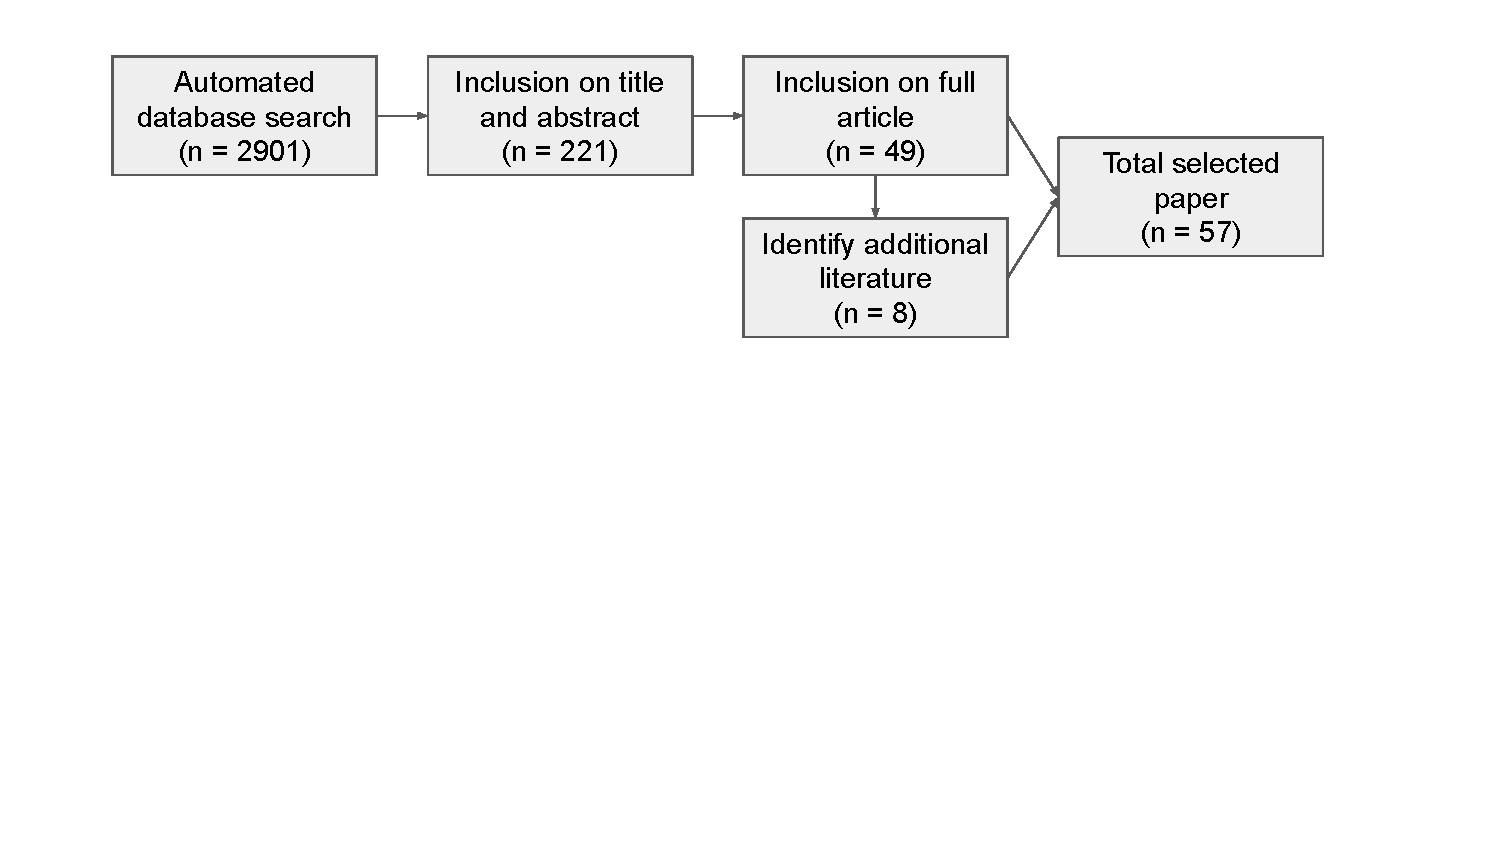
\includegraphics[width=1\columnwidth]{figures/fig-prisma.pdf}
  \caption{Literature search using PRISMA guidelines}
  \label{fig:prisma}
\end{figure}

\subsubsection*{Literature Corpus Characteristics}

The papers reviewed (n=57) were published between May 2011 and November 2022. More than 75\% of the papers were published in or after 2019, with a slight trend upwards over the years (see Figure \ref{fig:paper}). The vast majority of the papers in our corpus were published in conference proceedings (n=50), with the remainder papers published in journals. Out of the papers published in conferences, the top conferences were The ACM Conference on Human Factors in Computing Systems\footnote{https://dl.acm.org/conference/chi} (n=16), Conversational User Interfaces\footnote{https://dl.acm.org/conference/cui} (n=7), Human-Agent Interaction\footnote{https://dl.acm.org/conference/hai} (n=4), and Intelligent Virtual Agents\footnote{https://dl.acm.org/conference/iva} (n=4). 
%Out of the papers published in journals, some venues include the International Journal of Human-Computer Interaction\footnote{https://www.tandfonline.com/journals/hihc20} (n=2) and Interacting with Computers\footnote{https://academic.oup.com/iwc} (n=1).

On the modality characteristics of the conversational agents in the corpus, there is a roughly even split between the modalities, with slightly more papers exploring voice-based CAs (n=30) compared to text-based CAs (n=27).

%% Number of papers by year figure %%

\begin{figure}[h]
  \centering
  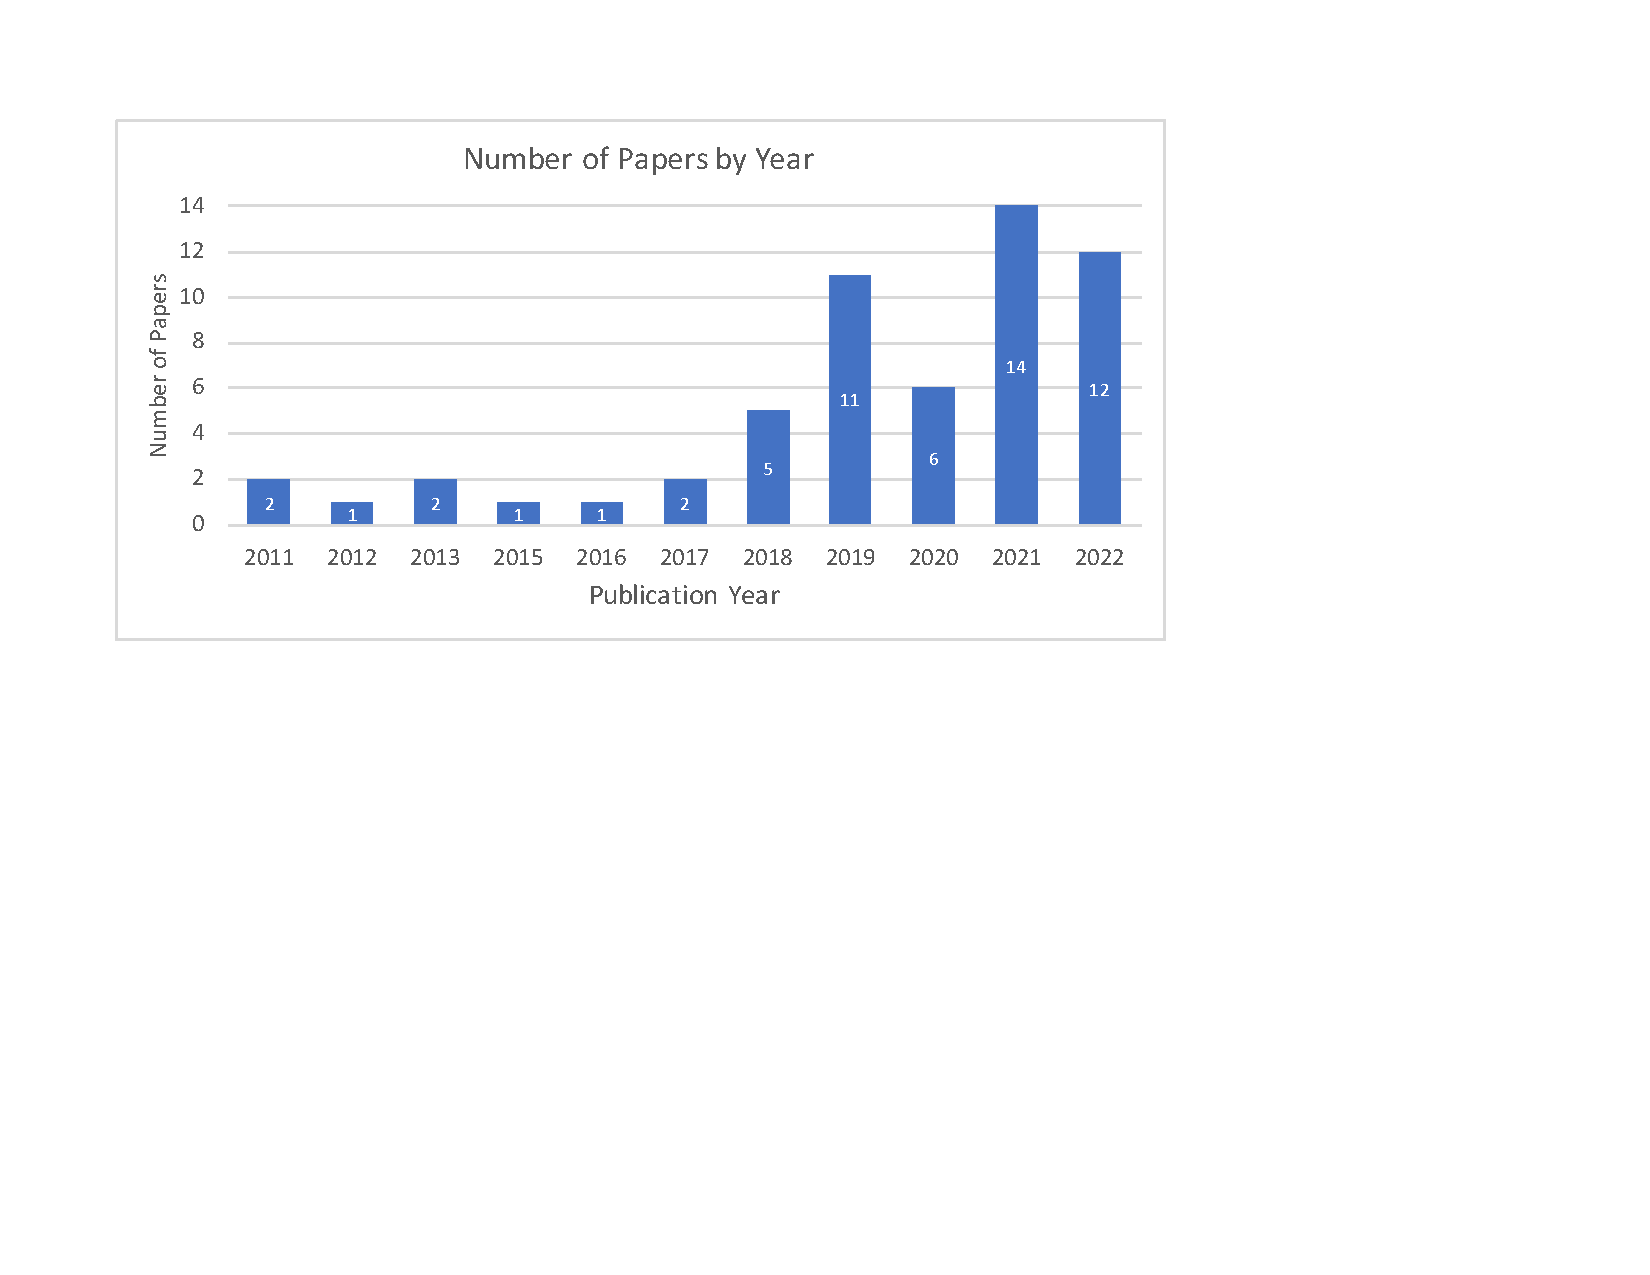
\includegraphics[width=\columnwidth]{figures/fig-paper.pdf}
  \caption{Number of papers by year}
  \Description{This graph shows the number of publications by year in our reviewed corpus between 2011 to 2022. There is a small number of papers each year between 2011 to 2017, with more papers per year starting in 2018. There is an upward trend on the number of publications over the years.}
  \label{fig:paper}
\end{figure}

\subsection{Data Analysis}

\subsubsection*{Perceptions of Agents} To understand the perceptions of agents related to conversation architecture (RQ1), assessments for the perceptions of agents were extracted from each paper. We used inductive thematic analysis to group these assessments into codes based on their meanings. For example, the code likeability of the agent contains the questionnaire item "this voice agent was likeable" used by \cite{cuadra2021my}\cmt{[67]}, Godspeed questionnaire \cite{bartneck2009measurement}\cmt{godspeed}'s set of questions on likeability used by \cite{linnemann2018can}\cmt{[15]}, and Subjective Assessment of Speech System Interface (SASSI) questionnaire \cite{hone2000towards}\cmt{sassi}'s set of questions on likeability used by \cite{chan2021kinvoices}\cmt{[74]}\cite{choi2020nobody}\cmt{[54]}. This step resulted in 83 unique codes. These codes are then organized based similarity of the meanings, resulting in 11 aspects of perceptions. For example, the aspect of personality traits of the agent contains measurements such as likeability, funniness, and kindness. Lastly, the 11 aspects are grouped into 4 categories: perception of interaction with agent, perception of agent's ability, perception of sociability with agent, and perception of agent's humanness (Table \ref{tbl:perceptions}).

\subsubsection*{Conversation Architecture Elements}
As to the elements of conversation architecture that are relevant to the perception of agents (RQ2), we extracted the specifics of conversation architecture used in each paper. Some of the papers used multiple features in their CA design, such as the the anthropomorphic agent used in Seeger et al's study \cite{seeger2021chatbots}\cmt{[35]}. In these composite situations, we broke them down into their individual features. For example, the anthropomorphic agent \cite{seeger2021chatbots}\cmt{[35]} was separated into emotional expressions, is-typing indicator, emoticons, and response delay and captured as codes. 58 unique codes were created as part of this process, capturing features like sentiment-adaptive responses \cite{diederich2019emulating}\cmt{[25]}, lexical alignment \cite{spillner2021talk}\cmt{[18]}, and typos \cite{westerman2019believe}\cmt{[9]}. We then organized these codes into elements based on similarity, resulting in 12 elements of conversation architecture. For example, the element of disfluency contains fillers \cite{jeong2019exploring}\cmt{[10]}\cite{wester2015artificial}\cmt{[14]}, interjections \cite{ceha2022expressive}\cmt{[77]}\cite{hu2021enhancing}\cmt{[56]}, repetitions \cite{yang2021effect}\cmt{[72]} and typos \cite{westerman2019believe}\cmt{[9]}. These elements are grouped into 4 categories: dialog strategy, content affectiveness, content style, and speech format (Table \ref{tbl:conversation_architecture}).

\subsubsection*{Relationship Between Perceptions of Agents and Conversation Architecture}

%% Heatmap of the identified relationships between perceptions & conversation architecture

\begin{figure*}[]
  \centering
  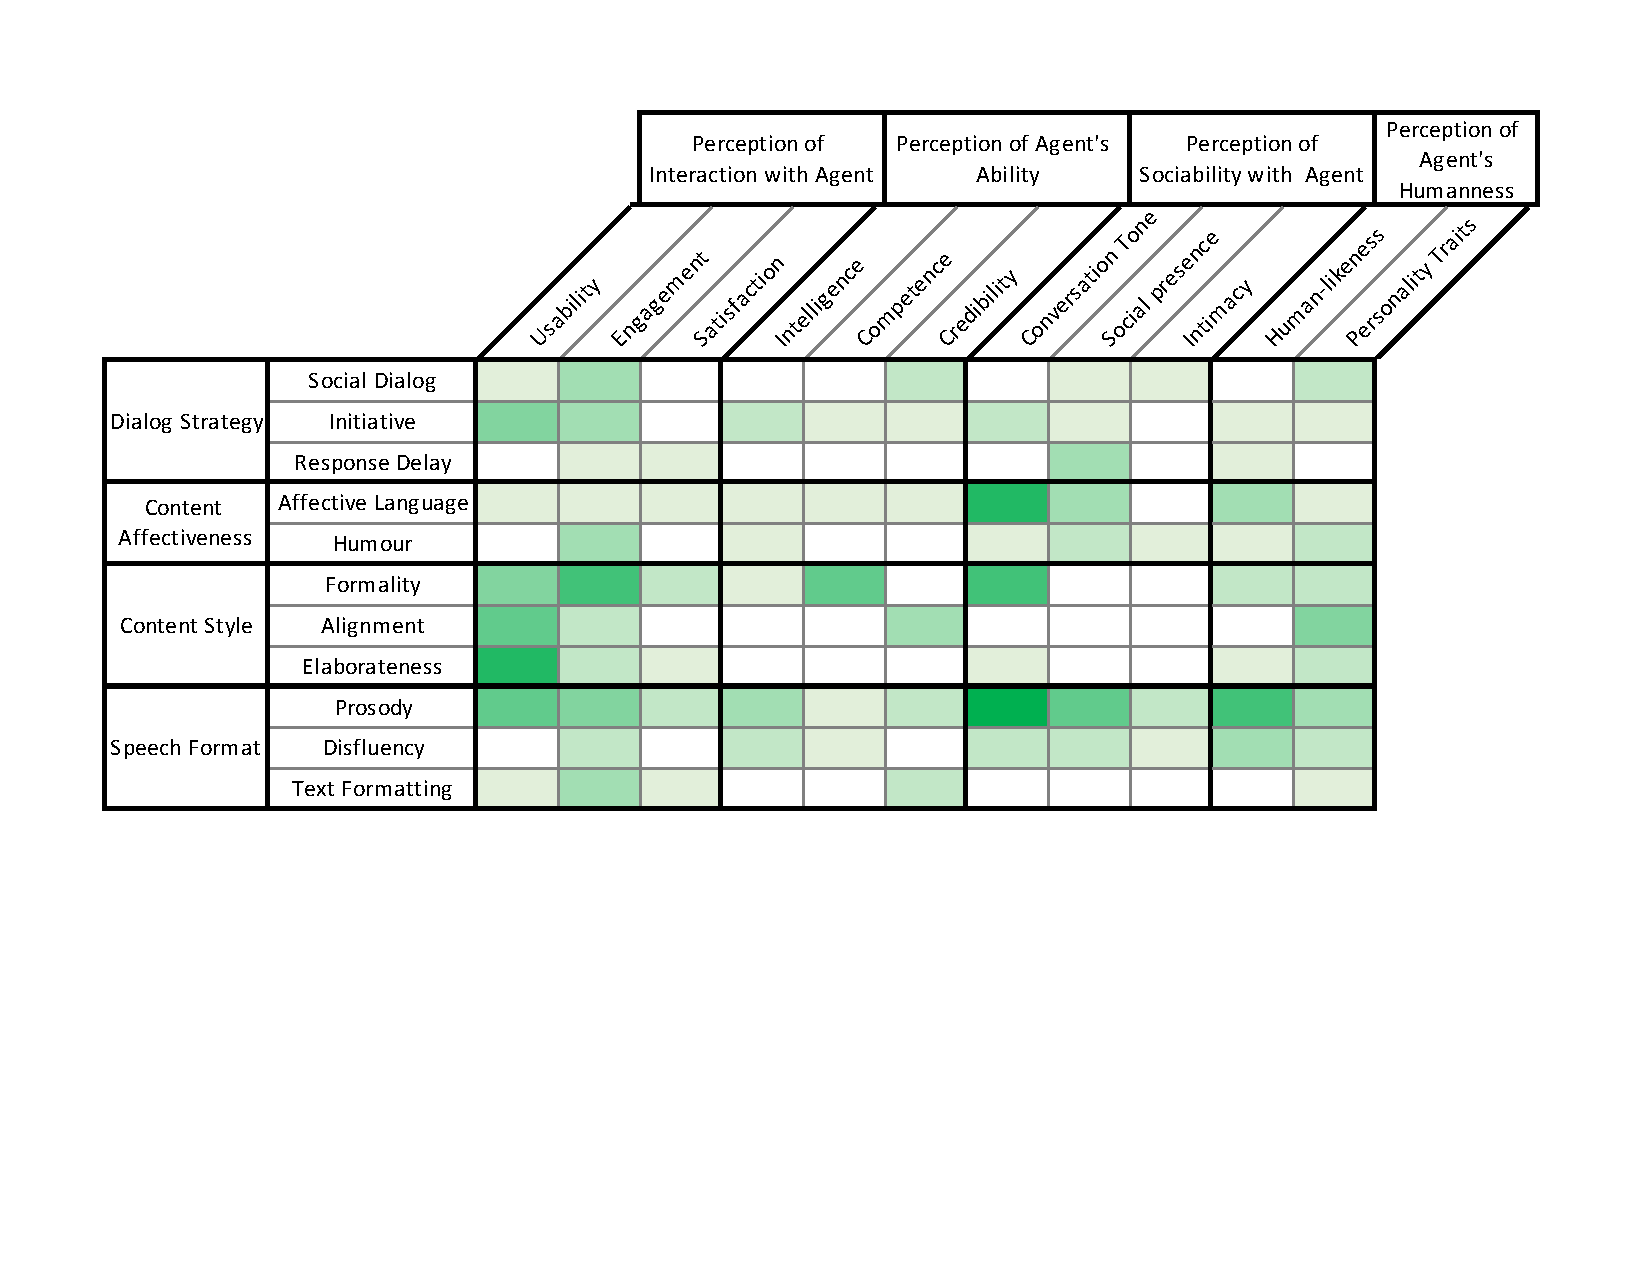
\includegraphics[width=\textwidth]{figures/fig-heatmap_identified.pdf}
  \caption{Heatmap of literature for perception of conversational agents for each type of conversational architecture element}
  \label{fig:heatmap_identified}
\end{figure*}

To study the effect of conversation architecture on users' perceptions (RQ3), we extracted the connections explored in each paper, using the perception aspects and conversation architecture elements developed in the previous data analysis steps. Each connection's effect was also recorded based on whether an association was found in the study and the nature of that association. Out of our review corpus, 265 connections between perceptions of agents and conversation architecture were explored in literature. To analyze the specifics of conversation architecture that affect the perceptions of CAs, 72 connections that did not result in observed relationships were discarded, resulting in 193 relationships for analysis. For example, the connection between the matching style of a CA and user satisfaction was removed because Hoegen et al. \cite{hoegen2019end}\cmt{[31]} did not find a significant difference between the style matching agent and the non-style matching agent for overall interaction satisfaction. Out of the 193 relationships, 10 were relationships based on agents modifying multiple architecture elements (e.g. \cite{seeger2021chatbots}\cmt{[35]}\cite{volkel2021manipulating}\cmt{[68]}). They were not included in the final framework as we could not attribute the perceptions of agents to the underlying core elements. Overall, 183 relationships between individual architecture elements and perceptions of agents are incorporated into our synthesized framework, visualized as a heatmap to demonstrate their relationships with each other (Figure \ref{fig:heatmap_identified}).
%% FINDINGS %%

\section{Findings}

\subsection{Perceptions of Agents}


As shown in \autoref{tbl:perceptions}, we defined four categories for the perceptions of conversational agents covering 11 different aspects of perception. The details of each category and aspect are discussed below.


\textbf{Perception of interaction with agent} assesses the overall interaction quality between users and conversational agents. The three aspects in this perception category  are: usability, engagement and satisfaction. \textit{Usability} captures the utilitarian component of the interaction, whether it was accurate, easy to use, efficient or helpful. Some commonly used methods to evaluate usability include the response accuracy portion of the SASSI questionnaire \cite{hone2000towards}\cmt{sassi}, or the NASA Task Load Index (NASA-TLX) \cite{hart1988development}\cmt{nasa} for cognitive workload. Questions such as ``\textit{the system is easy to use}'' or ``\textit{it is easy to understand the agent}'' are also used to evaluate usability. \textit{Engagement} on the other hand captures users' emotional reactions to the CA, including whether they have enjoyed the conversation, or felt annoyed or frustrated with the interaction. Some commonly used methods to evaluate engagement include the annoyance portion of the SASSI questionnaire \cite{hone2000towards}\cmt{sassi}, and the Use Engagement Scale (UES) \cite{o2018practical}\cmt{ues}. Questions such as ``\textit{I enjoyed using the system}'' or ``\textit{I felt frustrated with the agent}'' are also used to evaluate engagement. Lastly, \textit{Satisfaction} captures users' overall satisfaction interacting with the agent. Questions such as ``\textit{the overall assessment of conversing with the CA was satisfactory}'' are used to evaluate this aspect of perception.


%% PERCEPTION ASPECTS TABLE %%

\begin{table*}[ht]
\renewcommand*{\arraystretch}{1.4}
\resizebox{\textwidth}{!}{%
\begin{tabular}{@{}p{0.17\textwidth} | p{0.12\textwidth} | p{0.20\textwidth} | >{\centering}p{0.09\textwidth} | p{0.42\textwidth} @{}}
%!{\vrule width 1.2pt} 
\Xhline{1.2pt}
\multicolumn{2}{l|}{\textbf{Perception Aspects}} & \textbf{Examples} & \textbf{No. Papers} & \textbf{Papers} 
\\ \Xhline{1.2pt}
\multirow{3}{*}{\parbox{0.17\textwidth}{Perception of \newline Interaction with Agent}}
    & Usability & accuracy, ease of use, \newline efficiency, helpfulness & 23 
    & \cite{ashktorab2019resilient}\cmt{[88]}\cite{ceha2022expressive}\cmt{[77]}\cite{chan2021kinvoices}\cmt{[74]}\cite{choi2020nobody}\cmt{[54]}\cite{cuadra2021my}\cmt{[67]}\cite{dubiel2020persuasive}\cmt{[60]}\cite{elsholz2019exploring}\cmt{[61]}\cite{haas2022keep}\cmt{[78]}\cite{habler2019effects}\cmt{[63]}\cite{healey2013relating}\cmt{[39]}\cite{hu2022polite}\cmt{[76]}\cite{huiyang2022improving}\cmt{[17]}\cite{jestin2022effects}\cmt{[81]}\cite{kim2019comparing}\cmt{[89]}\cite{kim2020can}\cmt{[24]}
    \cite{kraus2020effects}\cmt{[64]}\cite{linnemann2018can}\cmt{[15]}\cite{ma2022ask}\cmt{[29]}\cite{miehle2018exploring}\cmt{[51]}\cite{misu2011toward}\cmt{[83]}\cite{roy2021users}\cmt{[71]}\cite{spillner2021talk}\cmt{[18]}\cite{wilhelm2022keep}\cmt{[28]}
\\ \cline{2-5}
    & Engagement & enjoyment, annoyance, \newline desirable, intention to use  & 28
    & \cite{andrews2012system}\cmt{[38]}\cite{ceha2022expressive}\cmt{[77]}\cite{ceha2021can}\cmt{[57]}\cite{chan2021kinvoices}\cmt{[74]}\cite{cox2022does}\cmt{[27]}\cite{cuadra2021my}\cmt{[67]}\cite{elsholz2019exploring}\cmt{[61]}\cite{fadhil2018effect}\cmt{[52]}\cite{gnewuch2022opposing}\cmt{[20]}\cite{go2021conversational}\cmt{[80]}\cite{healey2013relating}\cmt{[39]}\cite{huiyang2022improving}\cmt{[17]}\cite{jestin2022effects}\cmt{[81]}\cite{kim2020can}\cmt{[24]}\cite{kim2019comparing}\cmt{[89]}
    \cite{lee2020hear}\cmt{[23]}\cite{linnemann2018can}\cmt{[15]}\cite{ma2022ask}\cmt{[29]}\cite{miehle2018exploring}\cmt{[51]}\cite{miyamoto2017improving}\cmt{[46]}\cite{moilanen2022measuring}\cmt{[82]}\cite{roy2021users}\cmt{[71]}\cite{spillner2021talk}\cmt{[18]}\cite{volkel2021examining}\cmt{[69]}\cite{volkel2022user}\cmt{[75]}\cite{xiao2021let}\cmt{[73]}\cite{yang2021effect}\cmt{[72]}\cite{zhu2022effects}\cmt{[26]}    
\\ \cline{2-5}
    & Satisfaction & service satisfaction, quality of interaction & 12
    & \cite{ceha2022expressive}\cmt{[77]}\cite{choi2020nobody}\cmt{[54]}\cite{diederich2019emulating}\cmt{[25]}\cite{elsholz2019exploring}\cmt{[61]}\cite{habler2019effects}\cmt{[63]}\cite{gnewuch2018faster}\cmt{[19]}\cite{hoegen2019end}\cmt{[31]}\cite{hu2022polite}\cmt{[76]}\cite{ma2022ask}\cmt{[29]}\cite{roy2021users}\cmt{[71]}\cite{wilhelm2022keep}\cmt{[28]}\cite{yang2017perceived}\cmt{[44]}
\\ \Xhline{1.2pt} 
\multirow{3}{*}{\parbox{0.16\textwidth}{Perception of Agent's Ability}}
    & Intelligence & knowledgeable, intelligent, expertise & 11
    & \cite{ashktorab2019resilient}\cmt{[88]}\cite{ceha2021can}\cmt{[57]}\cite{chan2021kinvoices}\cmt{[74]}\cite{cuadra2021my}\cmt{[67]}\cite{dubiel2020persuasive}\cmt{[60]}\cite{feijoo2021effects}\cmt{[70]}\cite{hu2021enhancing}\cmt{[56]}\cite{jeong2019exploring}\cmt{[10]}\cite{spillner2021talk}\cmt{[18]}\cite{volkel2022user}\cmt{[75]}\cite{yang2017perceived}\cmt{[44]} 
\\ \cline{2-5}
    & Competence & competent, appropriate & 6 
    & \cite{cox2022does}\cmt{[27]}\cite{kraus2020effects}\cmt{[64]}\cite{jestin2022effects}\cmt{[81]}\cite{lee2019s}\cmt{[55]}\cite{misu2011toward}\cmt{[83]}\cite{westerman2019believe}\cmt{[9]}
\\ \cline{2-5}
    & Trust & credibility, trustworthy, truthfulness, confidence & 15
    & \cite{andrews2012system}\cmt{[38]}\cite{chan2021kinvoices}\cmt{[74]}\cite{dubiel2020persuasive}\cmt{[60]}\cite{fadhil2018effect}\cmt{[52]}\cite{healey2013relating}\cmt{[39]}\cite{hoegen2019end}\cmt{[31]}\cite{huiyang2022improving}\cmt{[17]}\cite{jestin2022effects}\cmt{[81]}\cite{kraus2020effects}\cmt{[64]}\cite{lee2020hear}\cmt{[23]}\cite{linnemann2018can}\cmt{[15]}\cite{ma2022ask}\cmt{[29]}\cite{seeger2021chatbots}\cmt{[35]}\cite{tolmeijer2021female}\cmt{[62]}\cite{wilhelm2022keep}\cmt{[28]}    
\\ \Xhline{1.2pt} 
\multirow{3}{*}{\parbox{0.16\textwidth}{Perception of \newline Sociability with Agent}}
    & Conversation Tone & friendly, warm, empathetic, persuasive & 20 
    & \cite{ashktorab2019resilient}\cmt{[88]}\cite{chan2021kinvoices}\cmt{[74]}\cite{cox2022does}\cmt{[27]}\cite{cuadra2021my}\cmt{[67]}\cite{daher2020empathic}\cmt{[58]}\cite{diederich2019emulating}\cmt{[25]}\cite{dubiel2020persuasive}\cmt{[60]}\cite{healey2013relating}\cmt{[39]}\cite{hu2021enhancing}\cmt{[56]}\cite{hu2022polite}\cmt{[76]}\cite{jestin2022effects}\cmt{[81]}\cite{khooshabeh2011does}\cmt{[37]}\cite{kim2019comparing}\cmt{[89]}\cite{lee2019s}\cmt{[55]}\cite{miehle2018exploring}\cmt{[51]}
    \cite{moilanen2022measuring}\cmt{[82]}\cite{tolmeijer2021female}\cmt{[62]}\cite{yang2021effect}\cmt{[72]}\cite{yang2017perceived}\cmt{[44]}\cite{zhu2022effects}\cmt{[26]}
\\ \cline{2-5}
    & Social Presence & connectedness, familiarity, psychological distance & 18
    & \cite{ceha2022expressive}\cmt{[77]}\cite{ceha2021can}\cmt{[57]}\cite{chan2021kinvoices}\cmt{[74]}\cite{choi2020nobody}\cmt{[54]}\cite{cuadra2021my}\cmt{[67]}\cite{diederich2019emulating}\cmt{[25]}\cite{gnewuch2018faster}\cmt{[19]}\cite{gnewuch2018chatbot}\cmt{[21]}\cite{gnewuch2022opposing}\cmt{[20]}\cite{go2021conversational}\cmt{[80]}\cite{khooshabeh2011does}\cmt{[37]}\cite{kim2020can}\cmt{[24]}\cite{lee2019s}\cmt{[55]}\cite{lubis2019positive}\cmt{[43]}\cite{lubold2016effects}\cmt{[86]}
    \cite{ma2022ask}\cmt{[29]}\cite{niewiadomski2013laugh}\cmt{[85]}\cite{westerman2019believe}\cmt{[9]}    
\\ \cline{2-5}
    & Intimacy & intimate, rapport, quality of relationship & 7 
    & \cite{choi2020nobody}\cmt{[54]}\cite{khooshabeh2011does}\cmt{[37]}\cite{kim2020can}\cmt{[24]}\cite{lee2020hear}\cmt{[23]}\cite{linnemann2018can}\cmt{[15]}\cite{lubold2016effects}\cmt{[86]}\cite{westerman2019believe}\cmt{[9]}
\\ \Xhline{1.2pt}
\multirow{2}{*}{\parbox{0.16\textwidth}{Perception of Agent's Humanness}}
    & Human-likeness & human-like, natural, \newline artificial, machine-like & 20
    & \cite{ashktorab2019resilient}\cmt{[88]}\cite{ceha2021can}\cmt{[57]}\cite{chan2021kinvoices}\cmt{[74]}\cite{choi2020nobody}\cmt{[54]}\cite{cox2022does}\cmt{[27]}\cite{diederich2019emulating}\cmt{[25]}\cite{gnewuch2018faster}\cmt{[19]}\cite{haas2022keep}\cmt{[78]}\cite{hu2022polite}\cmt{[76]}\cite{jeong2019exploring}\cmt{[10]}\cite{jestin2022effects}\cmt{[81]}\cite{lubis2019positive}\cmt{[43]}\cite{ma2022ask}\cmt{[29]}\cite{misu2011toward}\cmt{[83]}\cite{niewiadomski2013laugh}\cmt{[85]}
    \cite{ouchi2019should}\cmt{[59]}\cite{seeger2021chatbots}\cmt{[35]}\cite{wester2015artificial}\cmt{[14]}\cite{westerman2019believe}\cmt{[9]}\cite{zhu2022effects}\cmt{[26]}    
\\ \cline{2-5}
    & Personality Traits & likeable, kind, witty, funny, creepy & 20
    & \cite{andrews2012system}\cmt{[38]}\cite{ceha2022expressive}\cmt{[77]}\cite{ceha2021can}\cmt{[57]}\cite{chan2021kinvoices}\cmt{[74]}\cite{cuadra2021my}\cmt{[67]}\cite{haas2022keep}\cmt{[78]}\cite{habler2019effects}\cmt{[63]}\cite{healey2013relating}\cmt{[39]}\cite{hu2022polite}\cmt{[76]}\cite{huiyang2022improving}\cmt{[17]}\cite{jeong2019exploring}\cmt{[10]}\cite{kim2019comparing}\cmt{[89]}\cite{lee2020hear}\cmt{[23]}\cite{linnemann2018can}\cmt{[15]}\cite{miehle2018exploring}\cmt{[51]}
    \cite{ouchi2019should}\cmt{[59]}\cite{volkel2021manipulating}\cmt{[68]}\cite{volkel2022user}\cmt{[75]}\cite{wester2015artificial}\cmt{[14]}\cite{zhu2022effects}\cmt{[26]} 
\\ \Xhline{1.2pt}
\end{tabular}%
}
\caption{Perception aspects}
\label{tbl:perceptions}
\end{table*}

\textbf{Perception of agent's ability} assesses the perceived capabilities of the agent. Unlike system capabilities that affect agent's performance, this perceived ability category captures perceptions of agents with equivalent system capabilities but varied conversation architecture elements. Specifically, \textit{intelligence} captures the agent's perceived expertise and knowledge, and it is commonly administered through the Godspeed questionnaire \cite{bartneck2009measurement}\cmt{godspeed} using the set of questions related to perceived intelligence. Also survey questions such as asking users about the agent's intelligence and domain knowledge are used to evaluate perceived intelligence. \textit{Competence} takes intelligence one step further by examining the agent's perceived ability to put its intelligence into practice. Surveys or qualitative feedback are usually used to assess if the agent is capable and competent, and whether users have confidence in the agent's ability to get the job done. Lastly, \textit{credibility} captures agent's perceived truthfulness, benevolence, and user's confidence in CAs. Some commonly used methods to evaluate trust include the Trust Propensity Scale \cite{mayer1999effect} and the Individualized Trust Scale (ITS) \cite{wheeless1977measurement}. Questions such as ``\textit{is the agent honest}'' and ``\textit{can I trust the agent with sensitive information}'' are also used to evaluate trust.

\textbf{Perception of sociability with agent} assesses the emotional connections that users have with conversational agents. This category includes the perception aspects of conversation tone, social presence and intimacy. \textit{Conversation tone} captures the affective impression of the agent's tone, such as empathy and expressiveness. Also, this aspect includes whether the tone used by the agent was perceived as friendly, polite or warm. \textit{Social presence} captures the sense of connectedness and psychological distance users have with an agent. This perception aspect also includes the sense of familiarity or similarity with the agent, and whether users feel the agent behaves like them or has similar attitudes to them. The aspect of \textit{intimacy} extends social presence into the realm of the quality of relationships with an agent. Some commonly used methods to assess intimacy include the set of social attraction questions from the interpersonal attraction questionnaire \cite{mccroskey1975development} and the quality of relationship inventory (QRI) \cite{pierce1997assessing}. These questionnaires include questions like ``\textit{I think the agent could be a friend of mine}'', or ``\textit{I feel we could establish a personal relationship with each other}''.

\textbf{Perception of agent's humanness} assesses the specifics of anthropomorphized perceptions of conversational agents. \textit{Human-likeness} captures whether the agent presented itself as natural and human-like, or artificial and machine-like. The Godspeed questionnaire \cite{bartneck2009measurement}\cmt{godspeed} set of questions related to anthropomorphism and the Ascent of Man scale \cite{kteily2015ascent} are commonly used methods to evaluate human-likeness. Survey questions with semantic scales such as ``\textit{human-like / machine-like}'' and ``\textit{artificial / natural}'' are also used frequently to assess this aspect of perception. \textit{Personality traits} captures the human characteristics that are attributed to the agent. This is commonly collected as qualitative feedback from users, commenting on whether the agent is extroverted or introverted, or its perceived personality such as likeable, funny or witty. Sometimes the Big-5 personality traits questionnaire \cite{gosling2003very} is used to map an agent's disposition on various personality dimensions.

There is good coverage across the four perception categories based on our reviewed corpus. The perception category of interaction with agent is most commonly explored in literature, followed by the perception category of sociability with agent. Some aspects of perception are under explored in literature, such as the perceived intimacy with a CA or the perceived competence of an agent. This may be due to the controlled lab settings for experiments, where participants are given defined scenarios for interaction. This type of environment is not conducive to forming relationships with a conversational partner, as noted by Linnerman et al. in their discussions \cite{linnemann2018can}\cmt{[15]}. The same factor could impact the assessment of an agent's perceived competence, as users may not feel comfortable assessing the expertise of their conversational partner. 

%% CONVERSATION ARCHITECTURE ELEMENTS TABLE %%

\begin{table*}[t]

\caption{Categories of the conversation architecture elements with examples and related papers identified from our review.}
\Description{This table categorizes conversation architecture elements into four categories, provides some examples for the element, and shows the number of papers as well as references to the papers in our reviewed corpus. The first category is dialog strategy, which contains the elements of social dialog, initiative and response delay. The second category is content affectiveness, which contains the elements of affective language and humour. The third category is content style, which contains the elements of formality, alignment and elaborateness. The fourth category is speech format, which contains the elements of prosody, disfluency, and text formatting.}
\resizebox{\textwidth}{!}{
\renewcommand*{\arraystretch}{1.4}
\begin{tabular}{@{}p{0.17\textwidth} | p{0.14\textwidth} | p{0.25\textwidth} | >{\centering}p{0.09\textwidth} | p{0.34\textwidth} @{}}
\Xhline{1.2pt}
\multicolumn{2}{l|}{\textbf{Conversation Architecture Elements}} & \textbf{Examples} & \textbf{No. Papers} & \textbf{Papers}
\\ \Xhline{1.2pt}
\multirow{3}{*}{Dialog Strategy} & Social Dialog & social talk, self-disclosure  & 7
& \cite{andrews2012system}\cmt{[38]}\cite{lee2020hear}\cmt{[23]}\cite{lubold2016effects}\cmt{[86]}\cite{moilanen2022measuring}\cmt{[82]}\cite{roy2021users}\cmt{[71]}\cite{volkel2021manipulating}\cmt{[68]}\cite{volkel2022user}\cmt{[75]}
\\ \cline{2-5}

& Initiative & proactive dialogue, conversation \newline repair & 4
& \cite{ashktorab2019resilient}\cmt{[88]}\cite{cuadra2021my}\cmt{[67]}\cite{kraus2020effects}\cmt{[64]}\cite{xiao2021let}\cmt{[73]}
\\ \cline{2-5}

& Response Delay & response delay, typing indicator & 4
& \cite{gnewuch2018faster}\cmt{[19]}\cite{gnewuch2018chatbot}\cmt{[21]}\cite{gnewuch2022opposing}\cmt{[20]}\cite{seeger2021chatbots}\cmt{[35]}
\\ \Xhline{1.2pt}

\multirow{2}{*}{Content Affectiveness} & Affective Language & emotional expressions, sentiment-adaptive responses & 11
& \cite{daher2020empathic}\cmt{[58]}\cite{diederich2019emulating}\cmt{[25]}\cite{healey2013relating}\cmt{[39]}\cite{hu2022polite}\cmt{[76]}\cite{lee2019s}\cmt{[55]}\cite{lubis2019positive}\cmt{[43]}\cite{moilanen2022measuring}\cmt{[82]}\cite{seeger2021chatbots}\cmt{[35]}\cite{volkel2022user}\cmt{[75]}\cite{yang2017perceived}\cmt{[44]}\cite{zhu2022effects}\cmt{[26]}
\\ \cline{2-5}

& Humour & humorous content, jokes & 6
& \cite{ceha2021can}\cmt{[57]}\cite{go2021conversational}\cmt{[80]}\cite{khooshabeh2011does}\cmt{[37]}\cite{miyamoto2017improving}\cmt{[46]}\cite{niewiadomski2013laugh}\cmt{[85]}\cite{volkel2021manipulating}\cmt{[68]}
\\ \Xhline{1.2pt}

\multirow{3}{*}{Content Style} & Formality & formal vs. casual, honorific \newline expressions & 9
& \cite{cox2022does}\cmt{[27]}\cite{elsholz2019exploring}\cmt{[61]}\cite{habler2019effects}\cmt{[63]}\cite{jestin2022effects}\cmt{[81]}\cite{kim2019comparing}\cmt{[89]}\cite{ma2022ask}\cmt{[29]}\cite{moilanen2022measuring}\cmt{[82]}\cite{ouchi2019should}\cmt{[59]}\cite{volkel2022user}\cmt{[75]}
\\ \cline{2-5}

& Alignment & content matching, lexical \newline alignment, agreeableness & 7
& \cite{healey2013relating}\cmt{[39]}\cite{hoegen2019end}\cmt{[31]}\cite{huiyang2022improving}\cmt{[17]}\cite{linnemann2018can}\cmt{[15]}\cite{spillner2021talk}\cmt{[18]}\cite{volkel2021examining}\cmt{[69]}\cite{volkel2021manipulating}\cmt{[68]}
\\ \cline{2-5}

& Elaborateness & elaborate, concise, sentence \newline structure & 6
& \cite{haas2022keep}\cmt{[78]}\cite{miehle2018exploring}\cmt{[51]}\cite{moilanen2022measuring}\cmt{[82]}\cite{roy2021users}\cmt{[71]}\cite{volkel2021manipulating}\cmt{[68]}\cite{volkel2022user}\cmt{[75]}
\\ \Xhline{1.2pt}

\multirow{3}{*}{Speech Format} & Prosody & pitch, intonation, speech rate, \newline spoken accent & 12
& \cite{chan2021kinvoices}\cmt{[74]}\cite{choi2020nobody}\cmt{[54]}\cite{dubiel2020persuasive}\cmt{[60]}\cite{feijoo2021effects}\cmt{[70]}\cite{habler2019effects}\cmt{[63]}\cite{hu2021enhancing}\cmt{[56]}\cite{jestin2022effects}\cmt{[81]}\cite{kim2020can}\cmt{[24]}\cite{lubold2016effects}\cmt{[86]}\cite{misu2011toward}\cmt{[83]}\cite{tolmeijer2021female}\cmt{[62]}\cite{zhu2022effects}\cmt{[26]}
\\ \cline{2-5}

& Disfluency & fillers, interjections, repetitions, \newline typos & 6
& \cite{ceha2022expressive}\cmt{[77]}\cite{hu2021enhancing}\cmt{[56]}\cite{jeong2019exploring}\cmt{[10]}\cite{wester2015artificial}\cmt{[14]}\cite{westerman2019believe}\cmt{[9]}\cite{yang2021effect}\cmt{[72]}
\\ \cline{2-5}

& Text Formatting & capitalization, emoticons & 6
& \cite{fadhil2018effect}\cmt{[52]}\cite{kim2019comparing}\cmt{[89]}\cite{seeger2021chatbots}\cmt{[35]}\cite{volkel2022user}\cmt{[75]}\cite{westerman2019believe}\cmt{[9]}\cite{wilhelm2022keep}\cmt{[28]}
\\ \Xhline{1.2pt}
\end{tabular}%
}
\label{tbl:conversation_architecture}
\end{table*}

\subsection{Conversation Architecture Elements}

As shown in \autoref{tbl:conversation_architecture}, we defined four categories for conversation architecture across 11 different elements. The details of each category and element are discussed below.

The category of \textbf{dialog strategy} refers to the approach used by a conversational agent to engage in a dialogue with a user, which includes the use of social dialogs, agent-initiated content, and adding delays to responses. Specifically, the element of \textit{social dialogue} captures the use of non-task related conversations with users to build social connections, such as using self-disclosure \cite{lee2020hear}\cmt{[23]} and small talk \cite{lubold2016effects, volkel2021manipulating}\cmt{[86][68]}. The element of \textit{initiative} captures utterances that are initiated by an agent without direct prompts from users. For example, this element includes CAs designed to proactively initiate conversation repair \cite{ashktorab2019resilient, cuadra2021my}\cmt{[88][67]}, or actively elicit feedback from users \cite{xiao2021let}\cmt{[73]}. Lastly, \textit{response delay} refers to the tactic of deliberately delaying for a certain period of time before an agent responds to users \cite{gnewuch2018faster, gnewuch2022opposing}\cmt{[19][20]}. It is mainly used in text-based CAs alongside visual displays of typing indicators \cite{gnewuch2018chatbot}\cmt{[21]}.

\textbf{Content affectiveness} category refers to the conversational agent's use of language to convey emotions or to elicit emotions from users. The  element of \textit{affective language} captures injections of emotional words or phrases into an agent's utterances, such as the use of affective expressions \cite{seeger2021chatbots, yang2017perceived, zhu2022effects}\cmt{[35][44][26]}, sentiment-adaptive responses \cite{diederich2019emulating}\cmt{[25]}, and encouraging words \cite{healey2013relating}\cmt{[39]}. The other element in this category, \textit{humour}, captures an agent's attempt to include jokes in its dialog. Several studies in our reviewed corpus have explored the effect of humour on various perceptions of agents (e.g. \cite{ceha2021can, khooshabeh2011does}\cmt{[57][37]}).

The category of \textbf{content style} refers to the variations of language used in a message aside from the content meaning of the message (i.e. how something is said). The element of \textit{formality} describes the linguistic style used by a conversational agent, such as using formal language like honorific expressions to address users \cite{ouchi2019should}\cmt{[59]}. \textit{Alignment} captures the degree that an agent matches its utterances to users, such as being lexical aligned with the content and structure of users' sentences \cite{huiyang2022improving, linnemann2018can}\cmt{[17][15]}, as well as agreement with users \cite{volkel2021examining}\cmt{[69]}. Lastly, the element of \textit{elaborateness} captures the sentence complexity and length of agents' utterances. For example, \citet{roy2021users}\cmt{[71]} explored the differences in perceptions for elaborateness variations such as ``\textit{Cloudy, possibility of snow, high: 4, low: -10}'' vs. ``\textit{Today will be cloudy, with a high of 4 and a low of -10. Snow is predicted}''.

Lastly, the category of \textbf{speech format} refers to the non-verbal component of a conversational agent's utterances for both text and voice modalities. \textit{Disfluency} captures 
the use of non-lexical utterances like filler words (``\textit{um, uh}'') \cite{hu2021enhancing, jeong2019exploring}\cmt{[56][10]} or repetition of words within a sentence \cite{yang2021effect}\cmt{[72]}. It also includes the use of typos \cite{westerman2019believe}\cmt{[9]} for text-based agents. For voice-based agents specifically, the element of \textit{prosody} encompasses vocal qualities like pitch \cite{habler2019effects, jestin2022effects}\cmt{[63][81]}, speech rate \cite{choi2020nobody}\cmt{[54]}, and spoken accent \cite{feijoo2021effects}\cmt{[70]}. For text-based CAs, the \textit{text formatting} element includes different formats agents uses to present information to users, such as using capitalization \cite{westerman2019believe}\cmt{[9]} or emoticons \cite{kim2019comparing, wilhelm2022keep}\cmt{[89][28]}. 

Overall there are similar number of conversation architecture elements explored across the four categories of dialog strategy, content affectiveness, content style, and speech format. Looking across the 11 different elements of conversation architecture, there is a good coverage of studies on the effect of affective language and prosody cues on the perceptions of agents. However, there are less studies exploring the effect of agent initiated content and response delay on the perception of agents. Specifically for the element of agent initiated content, we found various research on conversation repairs \cite{komatani2010online, reinkemeier2022repair} and agents proactively sharing content with users \cite{dubiel2019inquisitive, zargham2022understanding}, but many of them did not not include assessments of users' perceptions of CAs. This may be due to the fact that the usage of agent-initiated content is relatively new, as CA interactions have historically been driven by users. As such, current research is focused on the functional aspects of agents initiating contents instead of exploring the perceptions of agents. As for response delay, our research suggests this element is under-explored in literature, as only 4 studies in our reviewed corpus examined agents using response delay, with majority of these publications published by the same authors.

\subsection{Relationship Between Perceptions of Agents and Conversation Architecture}

Our synthesized framework (\autoref{fig:heatmap_identified}) includes 183 identified relationships out of the 265 explored connections between perceptions of agents and conversation architecture elements. The differences between explored connections and identified relationships are shown as a side-by-side comparison in \autoref{fig:heatmap_coverage}, with detailed discussions in the subsections below.
%To compare the number of identified relationships vs. the explored connections in literature, \autoref{fig:heatmap_coverage} shows a side-by-side comparison between the two. The detailed analysis on the differences between explored and identified relationships are discussed in the subsections below.

%While the number of papers studying CAs with voice (n=27) vs. text (n=30) modalities is not significantly different, there are some interesting patterns with regards to the modalities of the identified relationships between perceptions of agents and conversation architecture. Overall, there are more explored conversation architecture elements related to voice-based CAs as compared to text-based CAs in the speech format category. Because there are smaller number of text-based CAs using speech format elements in our corpus, we also observed significantly smaller number of relationships between text-based CA across all perceptions of agents. Other interesting findings related to modality are discussed later in this paper.


%% Side by side comparison between coverage and identified relationships

\begin{figure*}[]
  \centering
  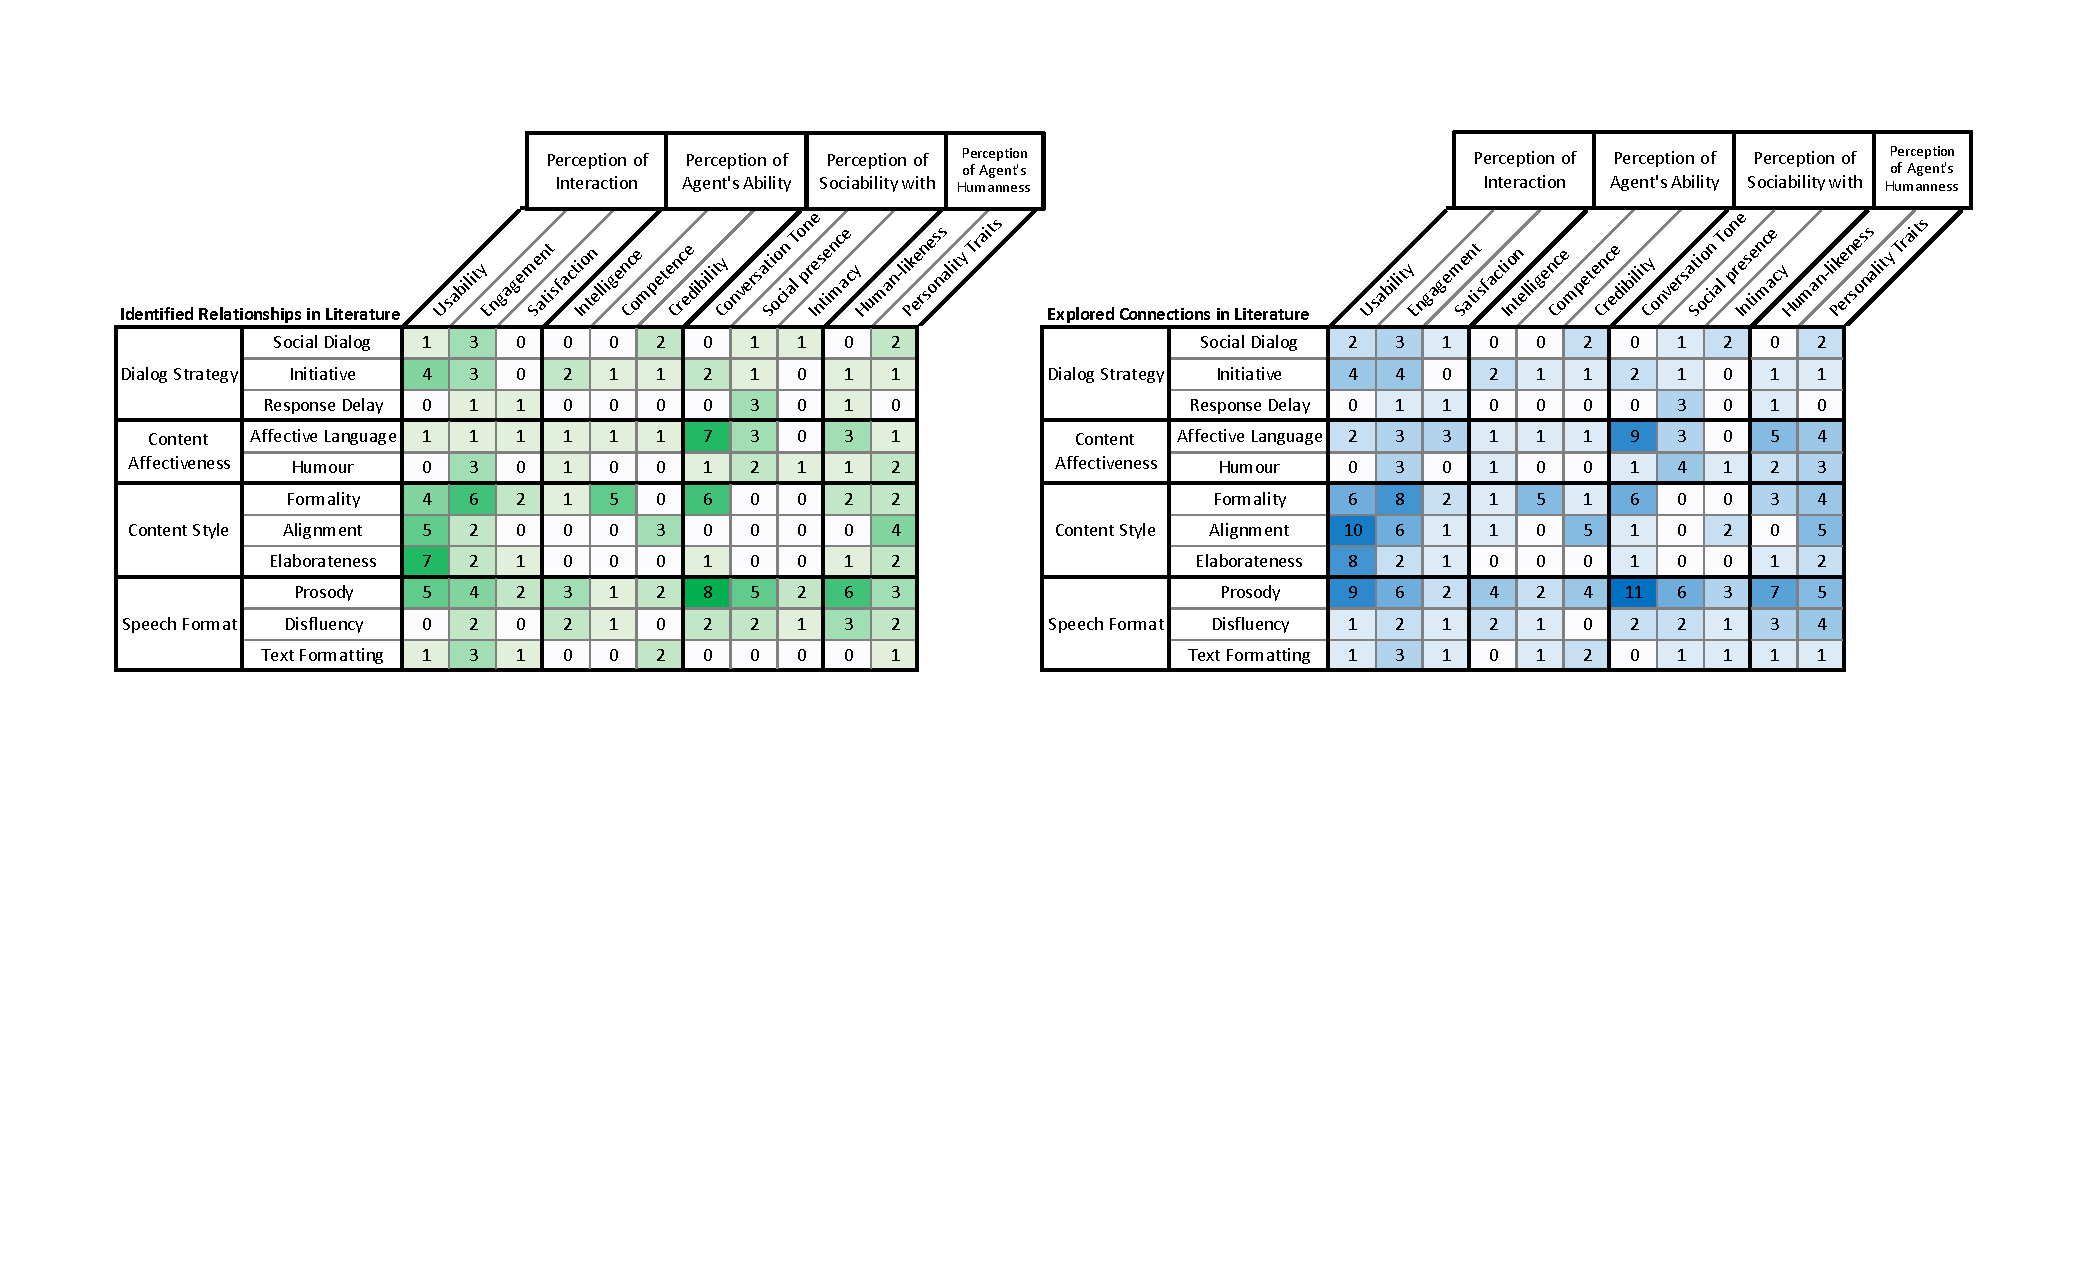
\includegraphics[width=\textwidth]{figures/fig-heatmap_coverage.pdf}
  \caption{Comparison between identified relationships and explored connections in literature}
  \Description{This figure shows a side by side comparison between the 183 identified relationships and the 265 explored connections in literature for conversation architecture elements and perceptions of agents. The visuals are shown as two heatmaps, with darker shades depicting higher number of relationships. The numbers within each cell at the interaction of a specific conversation architecture element and perception aspect outlines the number of relationships found in the reviewed corpus.}
  \label{fig:heatmap_coverage}
\end{figure*}

\subsubsection{Perception of Interaction with Agent}

The effects of conversation architecture elements on the perception of interaction with agent is the most explored connections in the corpus (n=97). Out of these explored connections, the majority of them (n=66) discovered relationships between the perceptions of interaction with agent related to the studied architecture element. Looking at the difference between modalities, we noticed more voice-based agents (n=25) resulted in null relationships compared to text-based agents (n=6). The conversation architecture element of \textit{alignment} contributed the most to the null results for voice-based agents, with 9 out of 11 explored connections not finding any relationships related the perception of interaction with agents.

Across the aspects for the perception of interaction, both usability and engagement were assessed frequently in our reviewed corpus, with speech variations having effects on both perception aspects across all conversation architecture element categories. The perception aspect of user satisfaction is commonly used to evaluate conversational agents within the customer service domain answering transactional inquiries (e.g. \cite{diederich2019emulating, elsholz2019exploring, gnewuch2018faster}\cmt{[25][61][19]}).

The category of conversation architecture with the most identified relationships to perceptions of interaction is content style. Specifically for the element of \textit{elaborateness}, users found the use of full sentences more useful than keyword only \cite{haas2022keep, roy2021users}\cmt{[78][71]}. Otherwise, the effect of an agent's elaborateness on user's perception of interaction depends on the user's preference \cite{miehle2018exploring}\cmt{[51]}, as well as the topic of discussion \cite{haas2022keep}\cmt{[78]}. As for \textit{formality}, various studies reported significant differences in the perceptions of interaction between CAs using casual vs. formal styles. However, there are mixed results on the effects on formality, as some users experienced higher engagement interacting with agent using casual style of conversation \cite{cox2022does}\cmt{[27]}, while in another study users found the CA using formal language style as less engaging as it is boring \cite{kim2019comparing}\cmt{[89]}.

There are also a number of papers in our reviewed corpus exploring the effect of speech format elements on the perception of interaction with CAs, with many of them finding significant relationships between them. The element with the most identified relationships is \textit{prosody}. For instance, studies found that a CA's expressiveness in vocal cues increased participants' engagement ratings \cite{zhu2022effects}\cmt{[26]}, and different pitches of voice affect users' perception of engagement and usability \cite{chan2021kinvoices, habler2019effects}\cmt{[74][63]}.

Dialog strategy and content affectiveness categories of conversation architecture did not have as many identified relationships with perceptions of interaction. It is worth noting the effect of using the \textit{initiative} element, as CAs that use self-initiated content are perceived as more efficient and higher quality of interaction \cite{cuadra2021my}\cmt{[67]}. Also, some studies have discovered conflicting effects between different perception aspects of interaction for CAs using \textit{social dialog}. One such example is users enjoying of the conversation with CAs using social talk \cite{lee2020hear, roy2021users}\cmt{[23][71]}, but perceiving the agent as less efficient \cite{roy2021users}\cmt{[71]}.

\subsubsection{Perception of Agent's Ability}

The effects of conversation architecture elements on the perception of agent's ability is the least explored connection in the corpus (n=39). Out of these explored connections, the majority of them (n=30) found relationships between the studied speech element and the perceptions of agent's ability. There are no notable differences between the text and voice modalities of CAs for either explored connections or the identified relationships.

Perception aspects of agent's ability had similar number of identified relationships with speech elements across intelligence, competence and credibility. Our review revealed that the perceived ability of a CA is also dependent on other influencing factors in addition to conversation architecture elements. For instance, \citet{kraus2020effects}\cmt{[64]} found that the perception of competence of a proactive CA is dependent on task difficulty. Also, the perception of intelligence for an agent using fillers depended on the context of the conversation, as the filler-speaking agent was perceived as less intelligent in task-oriented conditions, but was seen as slightly more intelligent in social-oriented conditions \cite{jeong2019exploring}\cmt{[10]}.

The conversation architecture element of \textit{prosody} has relationships identified with each perception aspect of an agent's ability. For example, Chan et al. \cite{chan2021kinvoices}\cmt{[74]} found that agents using kin's voices are rated as more intelligent and credible than generic voices. Also, the style of speech used by an agent affects the perception of appropriateness of tone, which is an aspect of the perceived competence of an agent \cite{misu2011toward}\cmt{[83]}. Different content styles of \textit{formality} used by a CA also impacts its perceived competence \cite{cox2022does, jestin2022effects}\cmt{[27][81]}. Related to the perception aspect of credibility, being \textit{lexically aligned} with the user improved the rating of trustworthiness of an agent \cite{hoegen2019end, linnemann2018can}\cmt{[31][15]}. There are some mixed results on the use of emoticons within the \textit{text formatting} element. One study found that chatbots using emoticons as less trustworthy \cite{wilhelm2022keep}\cmt{[28]}, while another study found that users assigned higher scores of confidence to the agent using emojis \cite{fadhil2018effect}\cmt{[52]}. 

There are several conversation architecture elements with little to no explorations related to the perception of agent's ability. Specifically, both categories of dialog strategy and content affectiveness are minimally explored in our reviewed corpus, with no explored connections with \textit{response delay} and only one or two connections explored for \textit{social dialog} and \textit{humour}. While some speech elements within the content style category have been evaluated for agents' perceived abilities, it is worth noting that the element of \textit{elaborateness} did not have any explored connections with perceived ability of agents. Further research in these areas is needed to close these knowledge gaps. 


\subsubsection{Perception of Sociability with Agent}

The perception of agent's sociability is the second most explored category within our reviewed corpus (n=64), with majority of the connections found relationships between the studied conversation architecture elements and perceptions of agent (n=49). Interestingly, studies explored more perceptions of sociability with agent related to voice-based CAs (n=40) compared to text-based CAs (n=24), potentially due to the assumption that interactions with text-based agents are perceived as less personal and more formal \cite{kocielnik2018designing}. There are some mixed results for voice-based CAs, as 12 out of the 28 explored connections did not find any significant results. Drilling down to the specific elements, we noticed that the use of \textit{alignment} in voice-based agents did not effect the perception of sociability with agent \cite{healey2013relating, linnemann2018can}\cmt{[39][15]}. As there are no papers in our reviewed corpus studying the effect of text-based agents using alignment on the perceptions of sociability, we were not able to compare the effect of alignment between modalities.

Across the aspects in this perception category, perceived conversation tone has the most number of identified relationship (n=27), followed by perceived social presence (n=17). There are only 5 relationships found between speech elements and perceived intimacy. One reason for this is half of the explored connections with speech elements did not have any effect on the perception of sociability with agent, such as the use of capitalization \cite{westerman2019believe}\cmt{[9]}, lexical alignment \cite{linnemann2018can}\cmt{[15]}, and social talk \cite{lubold2016effects}\cmt{[86]}. For the perception aspect of social presence, we noticed a gap exploring elements in the content style category (formality, alignment, elaborateness), as there are no connections explored at this intersection.

Looking at the different categories of conversation architecture elements, the heatmap (\autoref{fig:heatmap_identified}) shows that there are not many relationships in content style category of conversation architecture that are related to the aspects of perceived sociability with CAs. Most of the identified effects are concentrated at the intersection of \textit{formality} and perceived conversation tone. Studies have found that CAs using casual style of conversation are perceived as warm, empathetic and friendly \cite{jestin2022effects, kim2019comparing}\cmt{[81][89]}, while CAs using formal style of conversation are perceived as polite but lacks empathy \cite{cox2022does}\cmt{[27]}. The rest of the speech elements related to the perceptions of sociability are minimally explored in literature, indicating the need for more research in this area.

There are a few specific conversation architecture elements that has more identified relationships with perceptions of sociability with agent. Specifically, CAs using \textit{affective language} are perceived to be more empathetic \cite{daher2020empathic, diederich2019emulating, yang2017perceived}\cmt{[58][25][44]} and emotionally expressive \cite{zhu2022effects}\cmt{[26]}, as well as being more emotional connected with their users \cite{lee2019s, lubis2019positive}\cmt{[55][43]}. Also, different variations of a voice-based CA's \textit{prosody} have effects on the perceived sociability with agent, such as an agent using expressive prosody is assessed as more intimate and more similar with the user \cite{kim2020can}\cmt{[24]}. Lastly, the conversation architecture element of \textit{humour} has identified relationships across aspects of perceived sociability with CAs. Our review found that humor has effects on human-agent relationships, as humorous agents are rated as more friendly, intimate, and similar by users compared to non-humorous agents \cite{go2021conversational, khooshabeh2011does}\cmt{[80][37]}. This is contrary to \citet{clark2019makes}'s findings that while humour is an important conversational characteristic for human-human interactions, it is viewed as a novelty feature for human-agent conversations.


\subsubsection{Perception of Agent's Humanness}

There are 55 explored connections between conversation architecture elements and the perception of sociability with agents, with majority of them (n=38) discovering relationships in literature. There are significantly more explorations for voice-based agents (n=39) as compared to text-based agents (n=16). Previous studies have found that modality may have an effect on the perception of humanness, as voice-based agents are perceived as more human-like as compared to text-based agents \cite{cho2019effects}. Out of the 39 explored connections for voice-based agents, 14 of them did not result in any relationships. This is especially evident in the speech element of \textit{affective language} for voice-based agents, as most of the connections resulted in null relationships. For example, when comparing the ratings of human-likeness or likeability for a speech agent employing expressive words to the one not using any, Zhu et al \cite{zhu2022effects}\cmt{[26]} were unable to detect any statistically significant differences in both of the observation study and interaction study.

Across the aspects in this perception category, both human-likeness and personality traits have relationships with almost all the conversation architecture elements. Specifically for the use of \textit{prosody} in CAs, our review found some opposing effects on the perception of the agent's humanness. In the case of Chan et al's study \cite{chan2021kinvoices}\cmt{[74]}, participants rated the agent using kin voices as significantly more likeable compared to the generic voices, but it was perceived as eerie. This may be a warning indicator to beware of the uncanny valley effect \cite{mori2012uncanny} when designing conversation architecture elements to elicit anthropomorphized perceptions from users.

There are a few notable conversation architecture elements related to the perceived humanness of conversational agents. The element of \textit{prosody} such as varying pitch, intonation and speech rate has more identified relationships with perceived personality traits of an agent as compared to perceived human-likeness, especially on the perception of likeability for an agent \cite{choi2020nobody, jestin2022effects, misu2011toward}\cmt{[54][81][83]}. For the element of \textit{disfluency}, the effect on perceived humanness depended on the context of the conversation. Studies have found that participants perceived the filler-condition agent as more likeable in the social-oriented situation, but did not find the same effect in task-oriented situations \cite{jeong2019exploring, wester2015artificial}\cmt{[10][14]}. The use of \textit{alignment} in an agent has a number of identified relationships with the perception of personality traits of an agent, with some studies finding CAs that are lexically aligned with a user are more likeable \cite{huiyang2022improving, linnemann2018can}\cmt{[17][15]}. 
%% DISCUSSION SECTION %%

\section{Discussion}

\subsection{Research Challenges and Opportunities}

%Three major needs emerged from the trends identified by our review: 1) 2) 3).

\subsubsection{The Need for Consistent Evaluation Protocols for Perceptions of Agents}

We found a diversity of approaches used to assess perceptions of agents in our reviewed corpus. While we made our best efforts to group perceptions used in literature based on similarity with each other, the inconsistent and composite nature of these perception assessments makes it challenging to synthesize them into a framework that contains homogeneous components in each perception aspect that can be compared with each other.

Based on the literature reviewed in this paper, it is unclear whether perception aspects using similar labels are being evaluated \textit{consistently} through different approaches. For example, we found several methods used to assess the perceived human-likeness of an agent. A commonly used survey is adapted from the Godspeed questionnaire \cite{bartneck2009measurement}, which evaluates human-likeness based on users' impression of the agent as fake / natural, machinelike / humanlike, unconscious / conscious, and artificial / lifelike (used by \cite{hoegen2019end}\cmt{[31]}, \cite{jeong2019exploring}\cmt{[10]} and \cite{ouchi2019should}\cmt{[59]}). Another method used to evaluate human-likeness is adapted from Holtgraves et al.'s \cite{holtgraves2007perceiving} questionnaire, which asks users questions related to the agent's perceived human-likeness, skillfulness, thoughtfulness, politeness, responsiveness and engagement (used by \cite{diederich2019emulating}\cmt{[25]} and  \cite{gnewuch2018faster}\cmt{[19]}). One study \cite{westerman2019believe}\cmt{[9]} used the Ascend of Man scale \cite{kteily2015ascent} with pictures showing the evolution from ape to man, asking users to choose a depiction that best represents the agent's perceived human-likeness. It is unclear whether these different methods are capturing assessments of similar perception aspects that can be compared with each other. Another example is the evaluation of the perception of agent's empathy. In Diedrech et al.'s study \cite{diederich2019emulating}\cmt{[25]}, empathy is assessed by asking users whether the CA is giving users individual or personal attention. In another study that also studies the perception of empathy \cite{daher2020empathic}\cmt{[58]}, the RoPE Scale \cite{charrier2019rope} is used with questions like "the robot cares about my feelings" or "the robot comforts me when I am upset." These two different evaluations of empathy seem to have different underlying meanings, one assessing the personalization aspect of CAs, while the other is assessing the emotional aspect of CAs.

In addition the problem of consistency in evaluating perceptions, there is the issue of  \textit{composite measures} being used in the assessment of users' perceptions. These composite measures collapse multiple aspects of perception into one measurement, making it impossible to break down perceptions into more granular aspects for analysis. One such example is Ma et al's study \cite{ma2022ask}\cmt{[29]} on the different approaches for CAs to reply to users' uncertain queries. A single UX score is used to evaluate the users' perceptions, which composes of questions on whether the user thinks the CA's response is pleasing / trustworthy / natural / acceptable / shorten the distance between CA and the user. The UX score encompasses multiple aspects across several perception categories. While this study has found significant effect for the use of formal language on the user-rated UX score, it is not possible to understand how the details of formality is related to the perception categories of interaction (pleasing, acceptable), sociability (shorten the distance between CA and user), and humanness (natural, trustworthy). The humanness questionnaire from Holtgraves et al \cite{holtgraves2007perceiving} has a similar problem, evaluating across perception categories of interaction (responsiveness, engagement), ability (skillfulness), sociability (politeness), and humanness (human-likeness, thoughtfulness).

There has been some effort recently towards unifying the evaluation of conversational agents, such as the work by Finch et al. \cite{finch2020towards} presenting a comprehensive analysis of current evaluation protocols. More research is needed in this area to standardize the assessment of perceptions to make them consistent, granular, and comparable across literature.

\subsubsection{Investigate the Relationship Across Perception Aspects of Agents}

There is evidence in literature that perception aspects of agents have effects on each other. For instance, Moussawi et al. \cite{moussawi2021perceptions}\cmt{[36]} conducted a study to understand the correlations between different perceptions related to users' intention to adopt a conversational agent. Specifically, they found a correlation within the category of perceived ability, where an agent's perceived intelligence is positively correlated to the perceived initial trust of the agent. This study also found that users with higher perceived intelligence of an agent are more likely to attribute higher ratings for perceived human-likeness, as well as for the usability and engagement aspects in the perception category of interaction. Lastly, the authors found that perceived humanness have a positive impact on perceived enjoyment, which lead to higher intention to adopt the CA. This study outlines that the perception aspects identified in this paper are not independent of each other.

Correlations between perception aspects are discussed in a few of the papers we reviewed. One of the studies showed that the CA's perceived personality trait of agreeableness has an influence on the users' perception of credibility \cite{andrews2012system}\cmt{[38]}. Seeger et al's study found a similar correlation, where higher perceived anthropomorphism led to lower loss of trust \cite{seeger2021chatbots}\cmt{[35]}. There are also correlations between aspects found within the same perception category, such as a speech agent that is rated higher in perceived human-likeness was associated with higher likability ratings \cite{zhu2022effects}\cmt{[26]}. Also, within the perception category of social connection, one study found that social distance is positively related to perceived social attraction \cite{westerman2019believe}\cmt{[9]}.
 
These correlations demonstrate that some perception aspects have effects on each other, either within the same category or across different categories. While there are limited research into this area, further investigations are needed to understand the relationships between various perception aspects.


\subsubsection{Research Directions for the Effects of Conversation Architecture on Users' Perceptions}

Our synthesized framework (\autoref{fig:heatmap_identified}) lays the foundation in understanding the effect of conversation architecture on the perception of agents. It showcases the density of explored relationships between them, as well as highlighting areas that are under-explored. In order to continue building our knowledge, it is important to investigate further into the effect of contextual factors as well as multiple conversation architecture elements on users' perceptions.

There are a few \textit{under-explored areas} in our synthesized framework. The perception category of agent's ability has the least number of explored connections with conversation architecture compared to other perception categories. Specifically, more studies are needed to understand the effects of social dialog, response delay, humour and elaborateness on users' perceptions of agents' ability. For the perception category of sociability with agents, there is a general lack of explored connections with the conversation architecture category of content style, especially for alignment and elaborateness elements. Lastly, more studies on the effect of dialog strategy for conversation architecture elements of initiative and response delay on the perceptions of agents are needed.

Some studies have discussed how differences in \textit{contextual factors} resulted in variations in the perceptions of agents while using similar conversation architecture elements. One of the factors is users' experience with CAs, as Gnewuch et al. \cite{gnewuch2018faster}\cmt{[19]} found that experienced users perceived the agent with a response delay as lower in social presence because it is seen as inefficient to wait for the CA to respond, but novice users perceived higher social presence conversing with the CAs using response delays because it is more similar to conversations with human partners \cite{gnewuch2018faster}\cmt{[19]}. User characteristics is another factor, as the perceived trustworthiness of a style-matching agent depended on users' own conversational style \cite{hoegen2019end}\cmt{[31]}. Some other contextual factors that resulted in differences in perceptions of an agent include the purpose of conversation (e.g. transactional vs. social) \cite{jeong2019exploring}\cmt{[10]}, anonymity of the conversation \cite{lee2020hear}\cmt{[23]}, and the sensitivity of information discussed in the interaction \cite{cox2022does}\cmt{[27]}. A comprehensive review to identify these contextual factors as well as to understand their effects on the perceptions of agents across various conversation architecture elements would be useful to tailor CA design for specific situations. 

As we gain a better understanding of the effects of a single conversation architecture element on the perceptions of agents, we can extend the research to using \textit{multiple conversation architecture elements} in an agent. Several papers in our reviewed corpus incorporated composite elements in an agent, such as the design of an anthropomorphized chatbot using elements such as affective language, emoticons, and response delays to assess users' perceptions compared to a non-anthropomorphized chatbot \cite{seeger2021chatbots}\cmt{[35]}. In addition to exploring the combined effects of conversation architecture elements on users' perceptions, it would also be interesting to understand the relative importance of each element on perceptions. Some studies analyzed the effect of modifying conversation architecture elements individually, as well as their combined effect on user's perceptions (e.g. \cite{habler2019effects, lubold2016effects, zhu2022effects}\cmt{[63][86][26]}). Specifically, Habler et al. \cite{habler2019effects}\cmt{[63]} found that the effect of social dialog is higher than the effect of prosody on the perception of agents. 


\subsection{Ethical Considerations}

The designers of conversational agents need to consider ethical implications and potential negative impacts for users. This section discusses three main areas of concern related to the effect of conversation architecture on the perceptions of agents: gender stereotypes, influencing users' actions, and privacy concerns.

For the element of prosody, various studies in our corpus explored the effect of different pitches on the perceptions of agents. Even in studies that are not explicitly analyzing the effect of different gendered voices in an agent, possible stereotypes may still exist in the study. Based on our reviewed corpus, studies found that lower pitches commonly associated with men are considered to be more desirable and authoritative but less friendly \cite{jestin2022effects, tolmeijer2021female}\cmt{[81][62]}. For Dubiel et al's study \cite{dubiel2020persuasive}\cmt{[60]}, the agent with a lower mean pitch was selected as the more persuasive voice. These results may be demonstrating users' unconscious bias to select a male-sounding voice as more persuasive and authoritative over female-sounding voices that are commonly associated with higher pitches. While some guidelines recommend designing agents to be androgynous to avoid gender stereotypes \cite{ruane2019conversational}, there are limitations in creating gender-ambiguous voices. Currently, there are no defined guidelines on what is perceived as a gender-neutral voice \cite{jestin2022effects}\cmt{[81]}. There is also a lack of voice generators available to generate voices that are perceived as androgynous \cite{tolmeijer2021female}\cmt{[62]}.

Studies have demonstrated that conversation architecture elements can be used to design perceptions of agents to make CAs more persuasive. This opens up the ethical issue of influencing users' attitudes and behaviours through these persuasion techniques. In a study by Chan et al \cite{chan2021kinvoices}\cmt{[74]}, they found that CAs using kin's voices are perceived as more credible and likable, with a higher perceived social presence with the agent. These perceptions contribute to the agent being more engaging and persuasive, therefore people are more likely to comply with its requests. Andrew et al \cite{andrews2012system}\cmt{[38]} found that tailoring the personality of the CA to users will positively impact an agent's persuasiveness. These persuasion techniques can be beneficial to help users achieve their goals, but can also be used for harmful actions, such as trying to get users to believe in false information.

Another key area of concern is privacy. Given the natural language format of conversational agents, users may be disclosing more sensitive and personal information than needed for the interaction. In relationship to conversation architecture, using elements like self-disclosure and persuasive voice prosody settings could result in users perceiving higher trust with the agent, leading them to disclose more sensitive information  \cite{dubiel2020persuasive, lee2020hear}\cmt{[60][23]}. This can expose users to attacks, such as CAs using voice impersonation to ask for personal information for malicious intents \cite{chan2021kinvoices}\cmt{[74]}. Designing for perceptions of agents requires careful consideration of privacy issues including the sensitivity of the data, who has access to it, and how to protect against nefarious users.

\subsection{Limitations}

Our systematic literature review was limited to papers published in the ACM Digital Library between 2010 and 2022. We may have missed literature published outside this time period, as well as in other libraries. Also, most of the studies in our corpus are based on lab experiments using short interactions with users. The generalizability of these findings needs to be verified through longer-term engagements with conversational agents deployed in real-world situations. Lastly, research without empirical studies on the perception of agents is excluded based on our selection criteria. We may have missed some influential findings in these papers. %To better understand the relationships between conversation architecture elements and the perceptions of agents, we plan to conduct future reviews in literature and user studies to understand their real-world impacts.
%% CONCLUSION SECTION %%

\section{Conclusion}

In this paper, we share our findings of a systematic review of existing literature published in the ACM Digital Library on the effect of conversation architecture elements on the perceptions of CAs. Through the synthesis of 57 papers in our corpus, we found that current literature has explored users' perceptions of agents related to interaction, ability, sociability and humanness in relation to the effects of conversation architecture (RQ1). Also, we observed that conversation architecture elements related to dialog strategy, content affectiveness, content style, and speech format are relevant to users' perceptions of agents (RQ2). Based on our in-depth analysis, we present a framework outlining the identified relationships between elements of agents' conversation architecture and aspects of users' perception (RQ3). Our investigation also revealed the need for consistent protocols in evaluating perceptions of agents, as measurements are inconsistent across studies. Also, more research is needed to investigate the under-explored areas in the framework, the relationship across perception aspects, the influence of contextual factors, and the effect of composite conversation architecture elements on users' perceptions. While our research contribute to the design of conversation architecture to orchestrate specific perceptions of agents, we urge designers to incorporate ethical perspectives into their design considerations, including potential gender stereotypes, the use of persuasive techniques to influence users, and privacy issues related to users disclosing sensitive information to agents.

%%
%% The acknowledgments section is defined using the "acks" environment
%% (and NOT an unnumbered section). This ensures the proper
%% identification of the section in the article metadata, and the
%% consistent spelling of the heading.
\begin{acks}
This work was supported by NAVER Corp.
\end{acks}


%%
%% The next two lines define the bibliography style to be used, and
%% the bibliography file.
\bibliographystyle{config/ACM-Reference-Format}
\bibliography{references}

%%
%% If your work has an appendix, this is the place to put it.
\appendix

%TC:ignore
\onecolumn
\section{Appendix}

% Please add the following required packages to your document preamble:
% \usepackage{booktabs}

\begingroup
\renewcommand{\arraystretch}{1.3}

\begin{longtable}{@{} | p{0.14\textwidth} | p{0.48\textwidth} | p{0.035\textwidth} | p{0.27\textwidth} | @{}}
\caption{Articles included in literature review} \\
\hline \textbf{Authors} & \textbf{Title} & \textbf{Year} & \textbf{Venue} \\ \hline
\endfirsthead

\multicolumn{4}{c}{{\bfseries \tablename\ \thetable{} -- continued from previous page}} \\
\hline \textbf{Authors} & \textbf{Title} & \textbf{Year} & \textbf{Venue} \\ \hline
\endhead

\endlastfoot

%Data
\citet{andrews2012system}\cmt{[38]} & 
  System personality and persuasion in human-computer dialogue & 
  2012 & ACM Transactions on Interactive Intelligent Systems (TiiS) \\ \hline 
\citet{ashktorab2019resilient}\cmt{[88]} &
  Resilient chatbots: Repair strategy preferences for conversational breakdowns &
  2019 & ACM Conference on Human Factors in Computing Systems (CHI) \\ \hline
\citet{ceha2022expressive}\cmt{[77]} &
  Expressive Auditory Gestures in a Voice-Based Pedagogical Agent &
  2022 & ACM Conference on Human Factors in Computing Systems (CHI) \\ \hline
\citet{ceha2021can}\cmt{[57]} &
  Can a Humorous Conversational Agent Enhance Learning Experience and Outcomes? &
  2021 & ACM Conference on Human Factors in Computing Systems (CHI) \\ \hline
\citet{chan2021kinvoices}\cmt{[74]} &
  KinVoices: Using Voices of Friends and Family in Voice Interfaces &
  2021 & ACM Conference on Computer Supported Cooperative Work (CSCW) \\ \hline
\citet{choi2020nobody}\cmt{[54]} &
  "Nobody speaks that fast!" An empirical study of speech rate in conversational agents for people with vision impairments &
  2020 & ACM Conference on Human Factors in Computing Systems (CHI) \\ \hline
\citet{cox2022does}\cmt{[27]} &
  Does Chatbot Language Formality Affect Users’ Self-Disclosure? &
  2022 & ACM Conference Conversational User Interfaces (CUI) \\ \hline
\citet{cuadra2021my}\cmt{[67]} &
  My bad! repairing intelligent voice assistant errors improves interaction &
  2021 & ACM Conference on Computer Supported Cooperative Work (CSCW) \\ \hline
\citet{daher2020empathic}\cmt{[58]} &
  Empathic chatbot response for medical assistance &
  2020 & ACM International Conference on Intelligent Virtual Agents (IVA) \\ \hline
\citet{diederich2019emulating}\cmt{[25]} &
  Emulating empathetic behavior in online service encounters with sentiment-adaptive responses: insights from an experiment with a conversational agent &
  2019 & International Conference on Computers and Information Systems (ICIS) \\ \hline
\citet{dubiel2020persuasive}\cmt{[60]} &
  Persuasive synthetic speech: Voice perception and user behaviour &
  2020 & ACM Conference Conversational User Interfaces (CUI) \\ \hline
\citet{elsholz2019exploring}\cmt{[61]} &
  Exploring Language Style in Chatbots to Increase Perceived Product Value and User Engagement &
  2019 & Conference on Human Information Interaction and Retrieval (CHIIR) \\ \hline
\citet{fadhil2018effect}\cmt{[52]} &
  The effect of emojis when interacting with conversational interface assisted health coaching system &
  2018 & EAI International Conference on Pervasive Computing Technologies for Healthcare (PervasiveHealth) \\ \hline
\citet{feijoo2021effects}\cmt{[70]} &
  Effects of Virtual Humans' Gender and Spoken Accent on Users' Perceptions of Expertise in Mental Wellness Conversations &
  2021 & ACM International Conference on Intelligent Virtual Agents (IVA) \\ \hline
\citet{gnewuch2018faster}\cmt{[19]} &
  Faster is not always better: understanding the effect of dynamic response delays in human-chatbot interaction &
  2018 & European Conference on Information Systems (ECIS) \\ \hline
\citet{gnewuch2018chatbot}\cmt{[21]} &
  The Chatbot is typing…'–The Role of Typing Indicators in Human-Chatbot Interaction &
  2018 & International Conference on Computers and Information Systems (ICIS) \\ \hline
\citet{gnewuch2022opposing}\cmt{[20]} &
  Opposing Effects of Response Time in Human-Chatbot Interaction &
  2022 & Business \& Information Systems Engineering (BISE) \\ \hline
\citet{go2021conversational}\cmt{[80]} &
  Conversational Agents Replying with a Manzai-style Joke &
  2021 & Australian Conference on Human-Computer Interaction (OzCHI) \\ \hline
\citet{haas2022keep}\cmt{[78]} &
  Keep it Short: A Comparison of Voice Assistants' Response Behavior &
  2022 & ACM Conference on Human Factors in Computing Systems (CHI) \\ \hline
\citet{habler2019effects}\cmt{[63]} &
  Effects of Smart Virtual Assistants' Gender and Language &
  2019 & Conference on Message understanding (MuC) \\ \hline
\citet{healey2013relating}\cmt{[39]} &
  Relating to speech evoked car personalities &
  2013 & ACM Conference on Human Factors in Computing Systems (CHI) \\ \hline
\citet{hoegen2019end}\cmt{[31]} &
  An End-to-End Conversational Style Matching Agent &
  2019 & ACM International Conference on Intelligent Virtual Agents (IVA) \\ \hline
\citet{hu2021enhancing}\cmt{[56]} &
  Enhancing the Perceived Emotional Intelligence of Conversational Agents through Acoustic Cues &
  2021 & ACM Conference on Human Factors in Computing Systems (CHI) \\ \hline
\citet{hu2022polite}\cmt{[76]} &
  Polite or Direct? Conversation Design of a Smart Display for Older Adults Based on Politeness Theory &
  2022 & ACM Conference on Human Factors in Computing Systems (CHI) \\ \hline
\citet{huiyang2022improving}\cmt{[17]} &
  Improving Interaction Experience through Lexical Convergence: The Prosocial Effect of Lexical Alignment in Human-Human and Human-Computer Interactions &
  2022 & International Journal of Human-Computer Interaction (IJHCI) \\ \hline
\citet{jeong2019exploring}\cmt{[10]} &
  Exploring effects of conversational fillers on user perception of conversational agents &
  2019 & ACM Conference on Human Factors in Computing Systems (CHI) \\ \hline
\citet{jestin2022effects}\cmt{[81]} &
  Effects of Wording and Gendered Voices on Acceptability of Voice Assistants in Future Autonomous Vehicles &
  2022 & ACM Conference Conversational User Interfaces (CUI) \\ \hline
\citet{khooshabeh2011does}\cmt{[37]} &
  Does it matter if a computer jokes &
  2011 & ACM Conference on Human Factors in Computing Systems (CHI) \\ \hline
\citet{kim2020can}\cmt{[24]} &
  "I Can Feel Your Empathic Voice": Effects of Nonverbal Vocal Cues in Voice User Interface &
  2020 & ACM Conference on Human Factors in Computing Systems (CHI) \\ \hline
\citet{kim2019comparing}\cmt{[89]} &
  Comparing Data from Chatbot and Web Surveys: Effects of Platform and Conversational Style on Survey Response Quality &
  2019 & ACM Conference on Human Factors in Computing Systems (CHI) \\ \hline
\citet{kraus2020effects}\cmt{[64]} &
  Effects of proactive dialogue strategies on human-computer trust &
  2020 & ACM Conference on User Modeling, Adaptation and Personalization (UMAP) \\ \hline
\citet{lee2019s}\cmt{[55]} &
  What’s on Your Virtual Mind? Mind Perception in Human-Agent Negotiations &
  2019 & ACM International Conference on Intelligent Virtual Agents (IVA) \\ \hline
\citet{lee2020hear}\cmt{[23]} &
  "I Hear You, I Feel You": encouraging deep self-disclosure through a chatbot &
  2020 & ACM Conference on Human Factors in Computing Systems (CHI) \\ \hline
\citet{linnemann2018can}\cmt{[15]} &
  ‘Can I Trust the Spoken Dialogue System Because It Uses the Same Words as I Do?’—Influence of Lexically Aligned Spoken Dialogue Systems on Trustworthiness and User Satisfaction &
  2018 & Interacting with Computers (IWC) \\ \hline
\citet{lubis2019positive}\cmt{[43]} &
  Positive emotion elicitation in chat-based dialogue systems &
  2019 & IEEE/ACM Transactions on Audio, Speech and Language Processing (TASLP) \\ \hline
\citet{lubold2016effects}\cmt{[86]} &
  Effects of voice-adaptation and social dialogue on perceptions of a robotic learning companion &
  2016 & ACM/IEEE International Conference on Human-Robot Interaction (HRI) \\ \hline
\citet{ma2022ask}\cmt{[29]} &
  Ask a Further Question or Give a List? How Should Conversational Agents Reply to Users' Uncertain Queries &
  2022 & International Journal of Human-Computer Interaction (IJHCI) \\ \hline
\citet{miehle2018exploring}\cmt{[51]} &
  Exploring the impact of elaborateness and indirectness on user satisfaction in a spoken dialogue system &
  2018 & ACM Conference on User Modeling, Adaptation and Personalization (UMAP) \\ \hline
\citet{misu2011toward}\cmt{[83]} &
  Toward construction of spoken dialogue system that evokes users' spontaneous backchannels &
  2011 & SIGdial Workshop on Discourse and Dialogue (SIGDIAL) \\ \hline
\citet{miyamoto2017improving}\cmt{[46]} &
  Improving Relationships Based on Positive Politeness Between Humans and Life-Like Agents &
  2017 & International Conference on Human-Agent Interaction (HAI) \\ \hline
\citet{moilanen2022measuring}\cmt{[82]} &
  Measuring the Effect of Mental Health Chatbot Personality on User Engagement &
  2022 & International Conference on Mobile and Ubiquitous Multimedia (MUM) \\ \hline
\citet{niewiadomski2013laugh}\cmt{[85]} &
  Laugh-aware virtual agent and its impact on user amusement &
  2013 & International Conference on Autonomous Agents and Multiagent Systems (AAMAS) \\ \hline
\citet{ouchi2019should}\cmt{[59]} &
  Should speech dialogue system use honorific expression? &
  2019 & International Conference on Human-Agent Interaction (HAI) \\ \hline
\citet{roy2021users}\cmt{[71]} &
  Users, Tasks, and Conversational Agents: A Personality Study &
  2021 & International Conference on Human-Agent Interaction (HAI) \\ \hline
\citet{seeger2021chatbots}\cmt{[35]} &
  Chatbots often Fail! Can Anthropomorphic Design Mitigate Trust Loss in Conversational Agents for Customer Service? &
  2021 & European Conference on Information Systems (ECIS) \\ \hline
\citet{spillner2021talk}\cmt{[18]} &
  Talk to Me on My Level-Linguistic Alignment for Chatbots &
  2021 & International Conference on Human-Computer Interaction with Mobile Devices and Services (MobileHCI) \\ \hline
\citet{tolmeijer2021female}\cmt{[62]} &
  Female by default?--exploring the effect of voice assistant gender and pitch on trait and trust attribution &
  2021 & ACM Conference on Human Factors in Computing Systems (CHI) \\ \hline
\citet{volkel2021examining}\cmt{[69]} &
  Examining User Preference for Agreeableness in Chatbots &
  2021 & ACM Conference Conversational User Interfaces (CUI) \\ \hline
\citet{volkel2021manipulating}\cmt{[68]} &
  Manipulating and Evaluating Levels of Personality Perceptions of Voice Assistants through Enactment-Based Dialogue Design &
  2021 & ACM Conference Conversational User Interfaces (CUI) \\ \hline
\citet{volkel2022user}\cmt{[75]} &
  User perceptions of extraversion in chatbots after repeated use &
  2022 & ACM Conference on Human Factors in Computing Systems (CHI) \\ \hline
\citet{wester2015artificial}\cmt{[14]} &
  Artificial personality and disfluency &
  2015 & INTERSPEECH \\ \hline
\citet{westerman2019believe}\cmt{[9]} &
  I Believe in a Thing Called Bot: Perceptions of the Humanness of “Chatbots” &
  2019 & Communication Studies \\ \hline
\citet{wilhelm2022keep}\cmt{[28]} &
  Keep on Smiling: An Investigation of the Influence of the Use of Emoticons by Chatbots on User Satisfaction &
  2022 & ACM Conference Conversational User Interfaces (CUI) \\ \hline
\citet{xiao2021let}\cmt{[73]} &
  Let Me Ask You This: How Can a Voice Assistant Elicit Explicit User Feedback? &
  2021 & ACM Conference on Computer Supported Cooperative Work (CSCW) \\ \hline
\citet{yang2021effect}\cmt{[72]} &
  The Effect of the Repetitive Utterances Complexity on User’s Perceived Empathy and Desire to Continue Dialogue by a Chat-oriented Dialogue System &
  2021 & International Conference on Human-Agent Interaction (HAI) \\ \hline
\citet{yang2017perceived}\cmt{[44]} &
  Perceived Emotional Intelligence in Virtual Agents &
  2017 & ACM Conference on Human Factors in Computing Systems (CHI) \\ \hline
\citet{zhu2022effects}\cmt{[26]} &
  Effects of Emotional Expressiveness on Voice Chatbot Interactions &
  2022 & ACM Conference Conversational User Interfaces (CUI) \\ \bottomrule
%\end{tabular}
\end{longtable}
\label{tab:appendix}
\endgroup
%TC:endignore



\end{document}
\endinput
%%
%% End of file `paper.tex'.